\documentclass{dsa-latex/newlayout}
%Bitte hier den enstprechenden Ort einsetzen z.B. Braunschweig und die Akademienummer
\Akademie{Braunschweig}{2014}{2}

\usepackage[english,ngerman]{babel}
\usepackage{dsa-latex/misc}
\usepackage{multicol}
\usepackage
	[
		style=authoryear-comp,
		backend=biber,
		maxbibnames=99,
		%citestyle=authoryear-icomp
	]
	{biblatex}
	\DeclareNameAlias{sortname}{last-first}
		%makes Lastname, Firstname in the bibliography
	\renewcommand{\labelnamepunct}{\addcolon\space}
		%includes colon after year in bibliograpy
		\renewcommand*{\multinamedelim}{;\space}
		%changes name delimiter in citations and bibliography to semicolon

\usepackage{epigraph}
	\setlength{\epigraphwidth}{0.75\textwidth}
	%for nice-looking epigraphs, e.g. at the beginning of chapters etc.
%\usepackage{amsmath}%wird automatisch durch newlayout.cls geladen
\usepackage{amsfonts}

\addbibresource{emile_library.bib}

%%%%%Mathe-Definitionen
\newtheorem{Def}{Definition}
\newtheorem{Sat}{Satz}
\newtheorem{Bew}{Beweis}

%%%%Ende Mathe-Definitionen

\begin{document}

 %   \input{titel}
 \setcounter{page}{3}

\setcounter{tocdepth}{1}
 \tableofcontents

   \setcounter{secnumdepth}{1}

\setcounter{page}{7}
\setcounter{chapter}{0}

%Angabe, bis zu welcher Stufe die sections im Text nummeriert werden sollen.
      \settocdepth{2}

\course{4}{Schule und Demokratie}%%%
 \begin{coursetitle}
   \centerline{Schule und Demokratie}
   \bigskip
   \Large \centerline{Inklusive Pädagogik und Deliberative Politik}
   \bigskip
  \includegraphics[width=.9\columnwidth]{img/kurslogo.jpg}
  \label{fig:meinbild}
   \bigskip
\end{coursetitle}
%\begin{dsafigure}
%\begin{center}
%\includegraphics[width=.9\columnwidth]{Titelbild-fehlt.png}
%\caption{meine Bildunterschrift}
%label{fig:meinbild}
%\end{center}
%\end{dsafigure}

\section{Einführung}
	%!TEX root=./Emile.tex
\section{Einführung}

In unserem Kurs wird das Unmögliche versucht:
Wir bauen Brücken, wo sie noch nie gebaut worden sind.
Am Anfang unserer Kursarbeit hatten wir 16 Autoren sowohl der Sozialwissenschaften als auch der Pädagogik und ein utopisches Ziel:
Alle miteinander zu verbinden.

Ein Grundproblem, das sich sowohl in den Sozialwissenschaften als auch der Pädagogik wiederfindet ist das der Organisation des menschlichen Zusammenlebens.
In unserem Kurs wurde diese Problematik, die sich in einer Demokratie ebenso wie in der Schule stellt, anhand eines Hauses veranschaulicht.

\begin{dsafigure}
	\begin{center}
	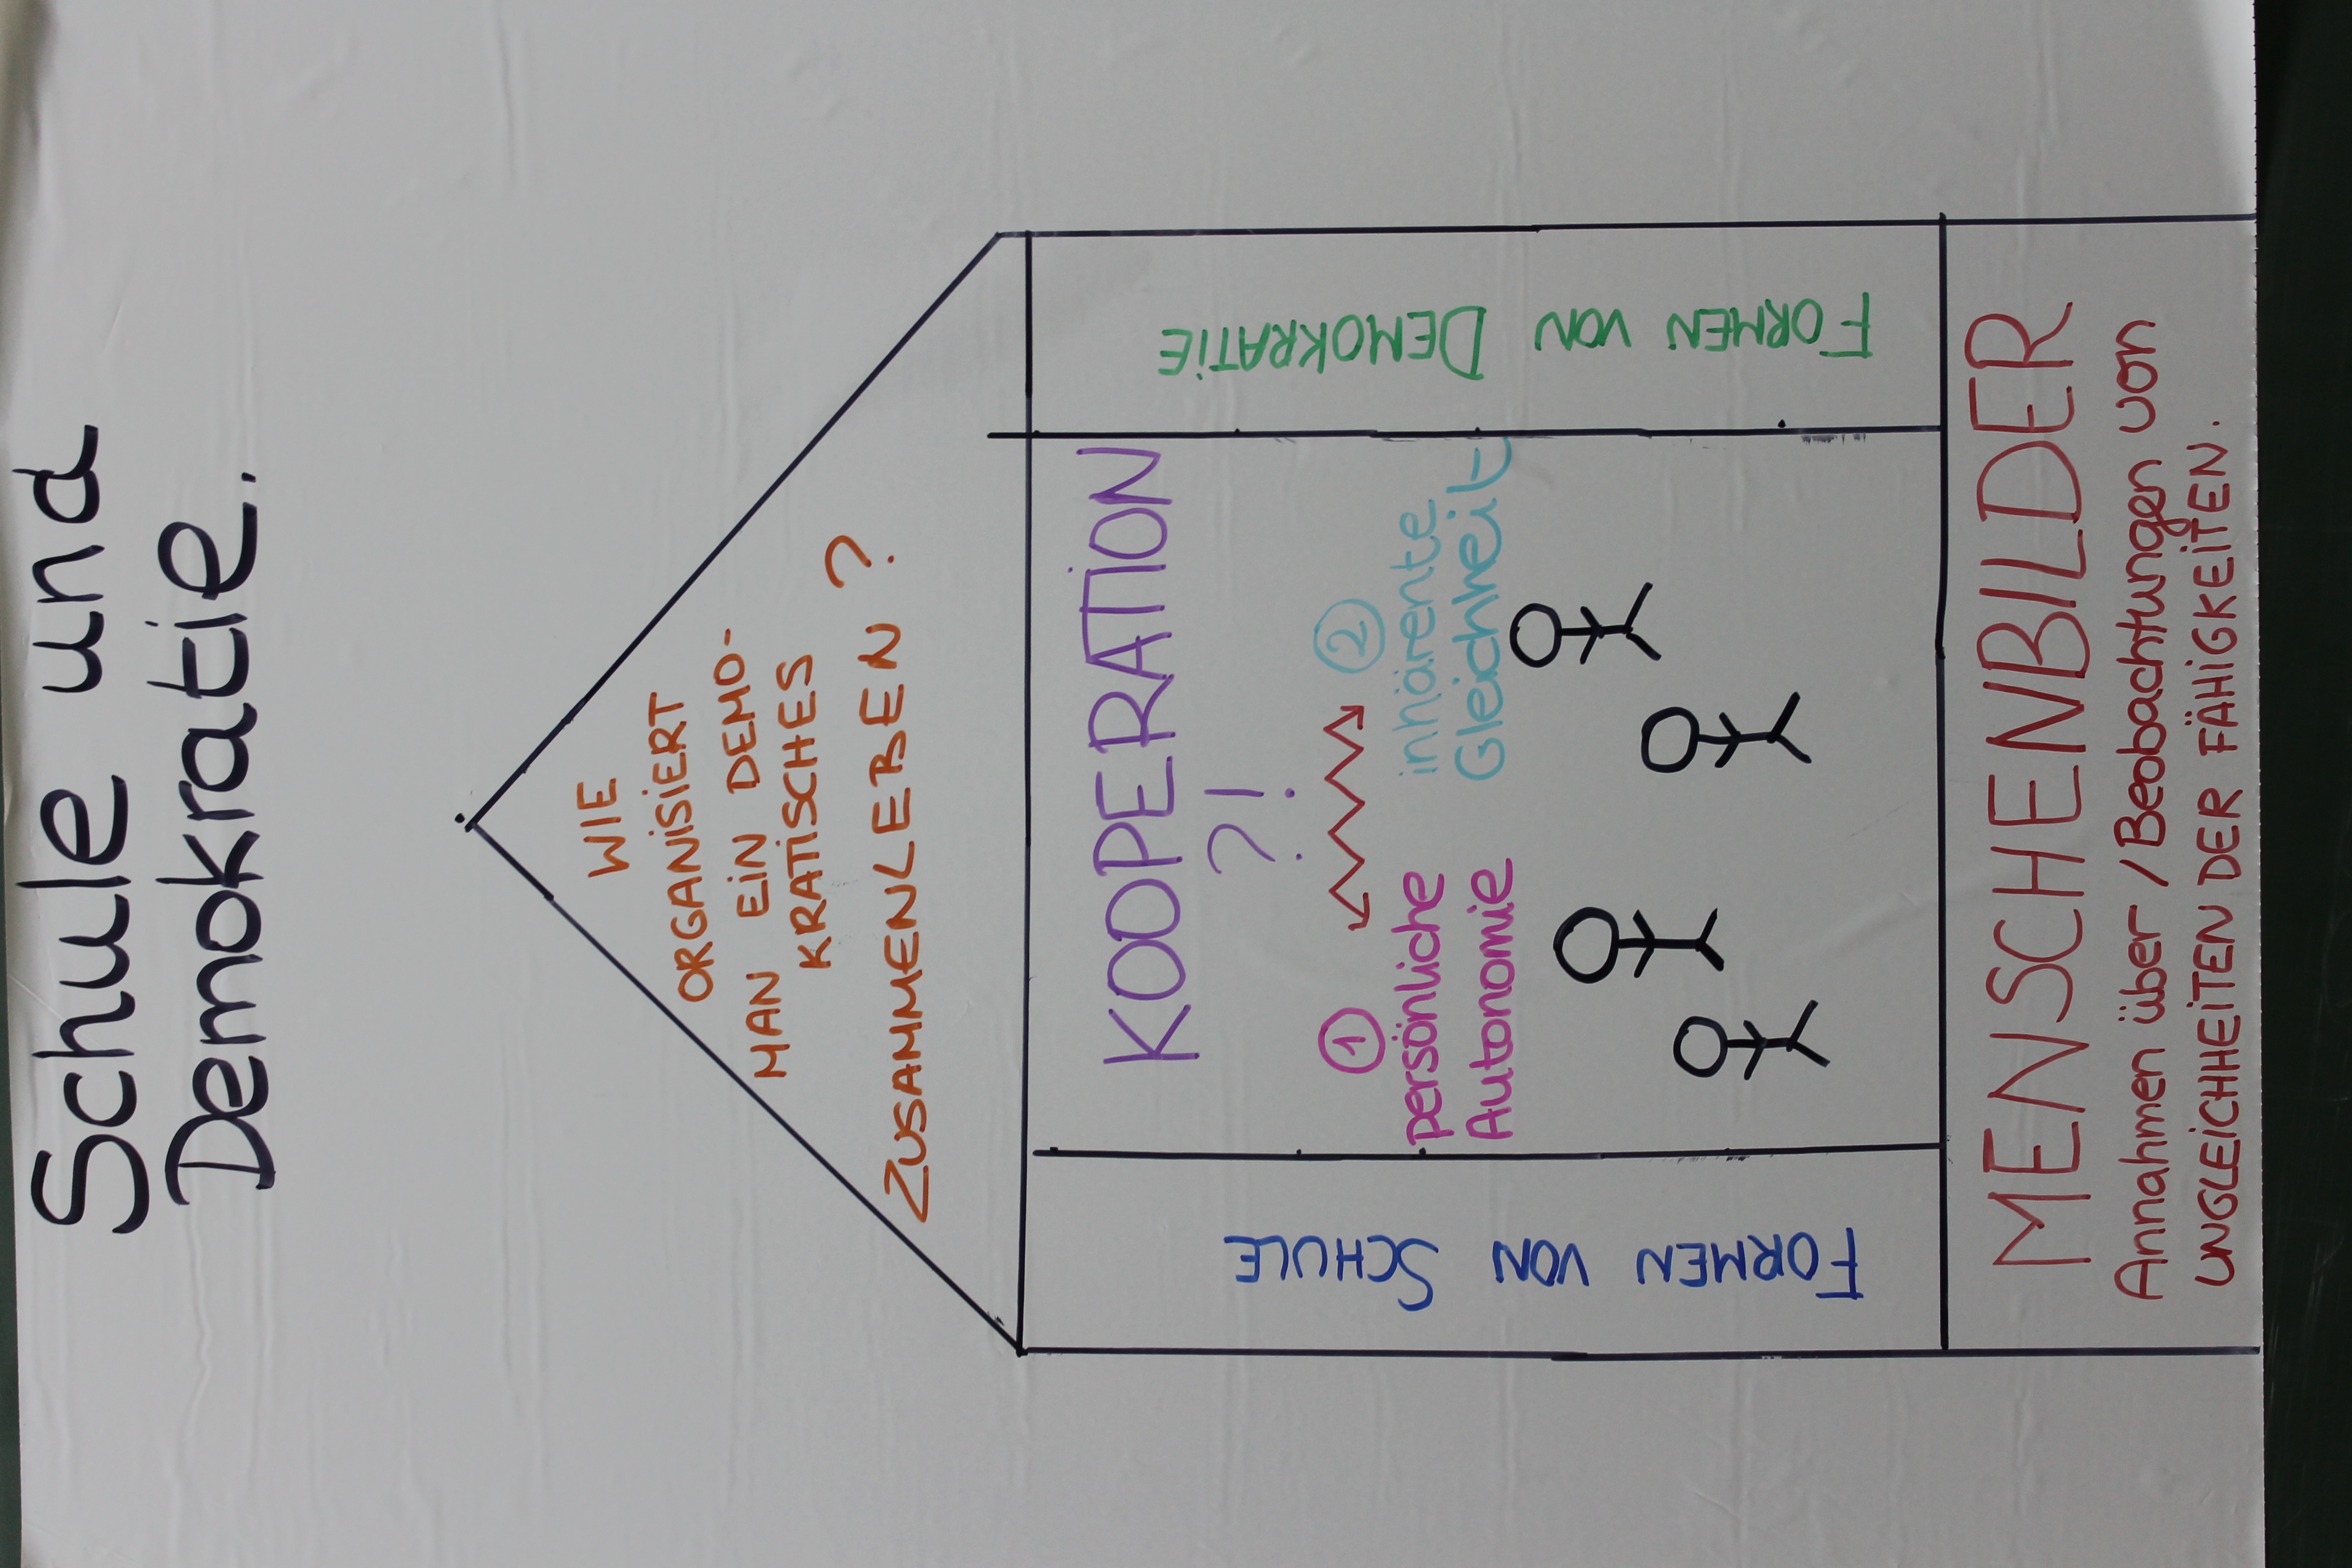
\includegraphics[width=0.9\columnwidth]{img/Kooperationshaus.JPG}
	\caption{Gemeinsame Fragen von Pädagogik und Sozialwissenschaft illustriert als Kooperationshaus}
	\label{fig:kooperationshaus}
	%\caption{Wie lässt sich menschliches Zusammenlebens bei beobachteter Ungleichheit organisieren? Ein Balanceakt zwischen inhärenter Gleichwertigkeit und persönlicher Autonomie}
	%MH FIXME: too long caption
	\end{center}
\end{dsafigure}

Nehmen wir an, dass der Mensch weder Herdentier noch Einzelgänger ist, sondern grundsätzlich in der Lage ist zu kooperieren.
Da aber (fast) jeder Mensch in eine Gesellschaft hineingeboren wird, ergibt sich zwangsläufig folgender Konflikt:
Inwiefern kann ein Mensch autonom über sich und sein Leben und Lernen entscheiden, ohne dabei die Entscheidungsfreiheit anderer und somit die inhärente Gleichheit, bzw. Gleichwertigkeit aller Menschen einzuschränken?
%VK: Ein Satz zur Kooperation ist notwendig! Ein Satz zu positiven Skalenerträgen (wird in den folgenden Beiträgen immer wieder erwähnt ohne Erklärung)

Die Aufgabe, die Balance zwischen persönlicher Autonomie und inhärenter Gleichheit zu finden, wird von unseren Autoren unterschiedlich gelöst.
Entsprechend unterschiedlich sind auch die Menschenbilder, die diesen Texten zugrunde liegen.
Sie bilden das Fundament unseres Hauses.

Den Herausforderungen des Zusammenlebens und -arbeitens nimmt sich dieser Kurs ganz konkret an:
Auf der Quellkontroll- und Versionsverwaltungsplattform \emph{github.com} versuchen wir uns an einem selbstorganisiertem Modus der Zusammenarbeit --- irgendwo zwischen Schule und Demokratie, zwischen Markt und Staat.
Dabei stellt sich uns immer wieder eine Frage:

\emph{Wie ist es also möglich, dass unterschiedliche und verschieden befähigte Menschen (auch wir auf der DSA) inhärent gleich und persönlich autonom zusammenleben?}

Unsere Einstellung zur Kursarbeit lässt sich durch ein Zitat von Martina Gedeck treffend beschreiben:

\begin{quote}
	``Im Leben geht es darum, die richtigen Fragen zu stellen und nicht darum, dauernd Antworten zu geben."\\*
	\emph{Martina Gedeck}
\end{quote}

Die richtige Frage ist gestellt, der Grundstein für unsere Brücken ist gelegt.
\section{Prolog}
	%!TEX root=./Emile.tex
\section[Prolog: Rousseau]{Prolog: Rousseaus idealistisches Gedankenexperiment}

\epigraph{
	``Man was born free and yet everywhere he lives in [chain stores].''\\*
	\emph{Jean-Jacques Rousseau / l`Internet}
}

Wie kann man Sozialwissenschaften und Pädagogik zusammen denken?
Wie persönliche Autonomie und inhärente Gleichheit verbinden?
Viele der Fragen, mit denen sich unserer Kurs beschäftigt, stellte sich Rousseau bereits im 18.\ Jahrhundert.
Auch wenn uns die Antworten, die er im \emph{Contrat Sociale} \parencite{Rousseau-1762-b} und dem Erziehungsroman \emph{Émile} \parencite{rousseau-1762} gibt, nicht unbedingt befriedigen mögen, so helfen sie doch zu präzisieren, wovon unser Kurs handelt.

\begin{dsafigurewide}[top]
	\begin{center}
	\includegraphics[width=.9\textwidth]{img/2014-2-4-Kursbild.jpg}
	\caption{Kurs 2.4}
	\label{fig:meinbild}
	\end{center}
\end{dsafigurewide}


\subsection{Émile: Oder über die Erziehung}

Rousseaus Gesellschaftsverständnis baut auf dem Menschenbild auf, das er in seinem Erziehungsroman Émile entwickelt:
Noch vor der französischen Revolution oder der Unabhängigkeitserklärung der Vereinigten Staaten stellt er, Bürger eines absolutistischen Feudalsystems, die These auf, jeder Mensch sei frei, persönlich autonom und inhärent gleichwertig.
Er schreibt: ``Der Mensch wird frei geboren, und überall ist er in Banden.'' \parencite[1]{Rousseau-1762-b}.
Doch wenn der Mensch nicht natürlich erzogen wird, werden diese Grundeigenschaften überdeckt.
Als Beispiel, wie diese natürliche Erziehung aussehen soll, legt Rousseau die Erziehung seines fiktiven Zöglings \emph{Émile} dar.

In der Kindheit wird der Junge, abgeschottet von der Gesellschaft, negativ erzogen.
Das heißt, das Kind lernt nichts über Moral, Religion oder Ethik, sondern es wird vor ``Laster[n] und [\ldots] Irrtümern bewahr[t]'' \parencite[54]{rousseau-1762}.
Anstelle dessen tritt eine Art ``Laissez-faire''-Pädagogik:
Wenn das Kind etwa von ihm benötigte Gegenstände zerstört,
``[b]eeilt euch nicht, ihm andere zu geben; laßt es empfinden, wie unangenehm es ist, sie nicht zu haben.'' \parencite[54]{rousseau-1762}.

Bis zum zwölften Lebensjahr soll das Kind auf diese Weise leben, stark und gesund werden.
Ab dann beginnt man, das Kind in Naturkunde zu unterrichten \parencite[55]{rousseau-1762}.
In diesem Unterricht aber hat die Lehrerin/Erzieherin\footnote{

	Im Folgenden verwenden wir die grammatikalisch weibliche Form.
	Gemeint sind immer Personen aller sozialen Geschlechter.
}
nur die Aufgabe, Lernsituationen zu schaffen.
Sie soll nichts erklären, sondern den Zögling allein herausfinden und verstehen lassen \parencite[56]{rousseau-1762}.

Erst wenn das Kind erwachsen wird, beginnt man mit der positiven Erziehung:
Das Kind wird nicht mehr als Zögling, sondern als Freund behandelt und moralisch, gesellschaftlich und religiös unterwiesen.
Es ist nun in der Lage, eigene fundierte Entscheidungen zu treffen --- wie etwa die Wahl seiner Religion \parencite[60f.]{rousseau-1762}.

Bald darauf kommt die Zeit, dass Émile in die Gesellschaft eingeführt werden muss, da der Mensch nicht für immer allein bleiben kann \parencite[61]{rousseau-1762}.
Der jetzt Erwachsene hat die Fähigkeit erworben, auch in der Gesellschaft seine Aufgabe zu erfüllen und trotzdem Mensch zu bleiben:

\begin{quote}
	``In der natürlichen Ordnung sind die Menschen alle einander gleich.
	Ihr gemeinsamer Beruf ist: Mensch zu sein.''\\*
	\parencite[50]{rousseau-1762}.
\end{quote}

Was passiert aber mit derjenigen, die nicht natürlich erzogen wird?

Ihre bürgerliche Erziehung zerteilt sie in verschiedene Rollen und Identitäten, deren verschiedenen Pflichten nicht miteinander zu vereinbaren sind.
Sie ist z.B.\ als Abgeordnete dem Fraktionszwang unterworfen, etwa für eine Steuer zu stimmen, und als Angehörige eines Berufsstandes muss sie dagegen sein.
Oder sie muss als Teilnehmerin der kursübergreifenden Musik (KüMu) zu einer Probe erscheinen und als Kursteilnehmerin Protokoll schreiben usw.
Dadurch, dass sie sich über verschiedene Aufgaben definiert, kann es leicht zu inneren Rollenkonflikten kommen.


\subsection{Le Contrat Social}

Während die bürgerlich Erzogene also in jeder ihrer Rollen \emph{Partikularinteressen} hat, kann ein natürlicher Mensch, der nur Mensch ist, das allgemeine menschliche Interesse des \emph{volonté générale} erkennen.
Rousseau geht davon aus, dass es im volonté générale (dem Gemeinwillen) ein vom Individuum losgelöstes abstraktes Wohl der Menschheit gibt.
Nur dieses Wohl könne in einem staatlichen System absolute Freiheit und Gleichheit garantieren.
Die problematische Vereinbarkeit von Freiheit und Gleichheit ergibt sich wiederum für Rousseau erst in der Moderne, da \emph{institutionalisierte}, rollengemäß ausdifferenzierte Kooperation den \emph{volonté générale} verdecken.
In der Moderne ist der Weg der Kooperation durch Traditionen, Gesetze oder anderes institutionalisierte Formen vorgeschrieben und definiert sich weniger zwischen natürlichen, \emph{ganzheitlichen} Menschen, sondern z.B.\ zwischen SchülerAkademie-Teilnehmenden (``TN'') und SchülerAkademie-Kursleitenden (``KL'').
Für Rousseau ist der Urzustand zwar das Optimum, jedoch ist dieser unwiederbringlich verloren.
Deshalb schlägt Rousseau den Weg über den volonté générale als Lösung vor.
Nur er kann und muss staatliche Gewalt rechtfertigen.

In einem so gelenkten Staat herrscht Gleichheit, da jedes Individuum und die Gesellschaft im Ganzen das Bestmögliche erhalten \parencite[7]{Rousseau-1762-b}.
Es herrscht gleichzeitig Freiheit, weil jedes Mitglied sich \emph{freiwillig} der Gemeinschaft unterordnet.
Im Zweifelsfall muss der Mensch jedoch auch dazu gezwungen werden, diese Freiheit wahrzunehmen.
Dabei gilt für ihn ``Each man [sic!] in giving himself to everyone gives himself to no one.'' \parencite[7]{Rousseau-1762-b}.
Er bleibt also vollkommen autonom.

Rousseau hat damit innerhalb seines Gedankenkonstrukts eine Lösung des Vereinbarkeitsproblems von Autonomie und Gleichwertigkeit gefunden.
Seine Intention lag dabei darin, ein normatives Gebilde zu errichten, nicht aber darin, eine Verfassung zu schreiben.
%MH TODO nochmal ausführen, welche verfassungsmäßigen Details hier etwa fehlen, und welche Konflikte (etwa Abstimmungsmodus) hier völlig unbearbeitet bleiben.
Dennoch hat er als erster Aufklärer, der etwa eine göttliche Herrschafts-Legitimation bestritt, großen Anteil an den freiheitlich demokratischen Entwicklungen der Folgezeit.

Rousseaus romantisch verklärten Ansichten erzeugen zwar einige Widersprüche, doch wir müssen festhalten, dass seine anti-modernen Ideen faszinieren und uns viele Anregungen für die weitere Arbeit mitgeben.

\section{Exposition}
	%!TEX root=../Emile.tex
\section[Exposition]{Exposition}

\subsection[Tilly]{Tilly: Staatsgenese als organisiertes Verbrechen}

\epigraph{
	``Homo homini lupus.''\\*
	\emph{\parencite{Hobbes-1651-aa}}
}

Bei genauerem Hinschauen erkennt man, dass das Kursthema voraussetzt, dass Demokratie überhaupt erstrebenswert ist.
Da kollektiv verbindliche Entscheidungen einer Demokratie inhärent sind, braucht man einen Staat, der diese unter Zwang durchsetzt.
Die Entstehung von Staaten ist das Thema Charles Tillys.
Staaten definiert er als die Kontrolle der physischen Gewalt über ein Volk auf einem zusammenhängenden Territorium:

\begin{quote}
	``national states: relatively centralized, differentiated organizations the officials of which more or less successfully claim control over the chief concentrated means of violence within a population inhabiting a large, contiguous territory.''\\*
	\parencite[170]{Tilly-1985-aa}.
\end{quote}


\paragraph{Wie entsteht ein Staat?}

Nach Tilly ist die Entwicklung eines Staates immer mit kriegerischen und gewaltvollen Handlungen verbunden.
Er geht sogar so weit zu behaupten, dass Gewalt notwendig für die Entwicklung eines Staates sei.
Der Ausgangspunkt für die Entwicklung eines Staates ist die Monopolisierung von Gewalt und Macht: ``governments organize and, wherever possible, monopolize violence'' \parencite[171]{Tilly-1985-aa}.
\citeauthor{Tilly-1985-aa} sagt, dass in der vor-staatlichen Zeit mehrere gewaltausübende Parteien konkurrierten.
Ähnlich einem \citeauthor{Hobbes-1651-aa}chen Urzustands, führt in diesem Wettbewerb jede Partei Krieg gegen jede \parencite{Hobbes-1651-aa}.
Dabei ist jene Person oder Gruppe im Vorteil, der es gelingt, positive Skalenerträge zu erzielen, also zu \emph{fallenden} Grenzkosten \emph{mehr} Gewalt (oder deren glaubhafte Androhung) zu produzieren.
Positive Skalenerträge entstehen, wenn die Kosten für die jeweils \emph{nächste} produzierte Einheit Gewalt sinken.
Tilly's konkurrierende Gewaltunternehmer versuchen sich durch technische oder organisatorische Innovationen einen Vorteil über die anderen Parteien zu verschaffen, um sich innerhalb eines geografischen Gebietes durchzusetzen \parencite[vgl.][173]{Tilly-1985-aa}.

\begin{dsafigure}
	\begin{center}
	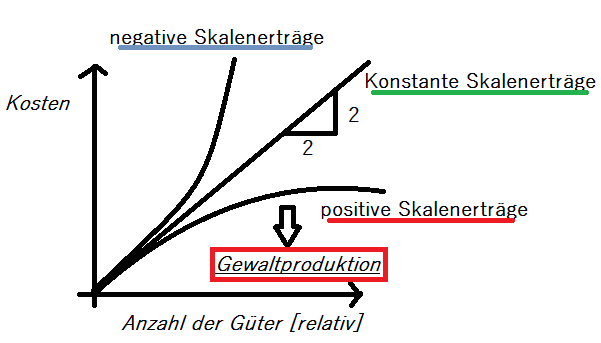
\includegraphics[width=0.9\columnwidth]{img/Skalenertraege.png}
	\caption{Positive Skalenerträge}
	\label{fig:skalenertraege}
	\end{center}
\end{dsafigure}

Für die herrschende Partei ist das ein Vorteil, da sie mit geringeren Kosten effizienter Gewalt ``produzieren'' kann.
Positive Skalenerträge kommen vor allem durch technische und organisatorische Innovationen zustande.
So ist beispielsweise bei niedrig entwickelten Waffen (wie Keulen) kaum ein solcher Vorteil erkennbar.
Es kostet einen bestimmten Geldbetrag, eine Keule herzustellen, die eine Person ausschalten kann.
Dieser Betrag bleibt auch bei den nächsten tausend produzierten Keulen ungefähr gleich.
Dadurch ergibt sich kein großer Vorteil.

Anders verhält es sich bei höher entwickelten Waffen wie der Wasserstoffbombe.
Hat diese bei einem Ertrag von mehreren Millionen Menschen, die auf einmal ausgeschaltet werden können, bei der ersten Herstellung noch extrem große Produktionskosten, so werden diese bei den nächsten produzierten Bomben deutlich kleiner.
Für die herrschende Partei stellt dies einen militärischen Vorteil dar.
Er kann mit höherer Produktion deutlich höhere Erträge bei gleichen Kosten erzielen und so die Konkurrenten ausschalten.

Positive Skalenerträge können damit erklären, wie aus vielen, relativ kleinen konkurrierenden Gewaltunternehmern (``Schutzgelderpressern''), effektive Monopolisten (``(National)staaten'') entstehen konnten.

Dieses Handeln ist entscheidend für die Entwicklung eines Staates, denn es zeigt, dass ein Staat nicht etwa infolge von friedlicher Zusammenarbeit der Menschen entsteht, sondern dieser materialistischen Theorie folgend an Machtkämpfe, Ausbeutung und Krieg gebunden ist: ``war making likewise led to state making'' \parencite[183]{Tilly-1985-aa}.

Durch sein Gewaltmonopol hat die herrschende Gruppe die Möglichkeit, von seinem Volk Tribute (Steuern) einzufordern und im Gegenzug \emph{Sicherheit} anzubieten: ``governments are in the business of selling protection'' \parencite[175]{Tilly-1985-aa}.
Allerdings funktioniert dies nur durch anhaltende Gewaltpräsenz und durch Drohungen des Herrschers.

\citeauthor{Tilly-1985-aa} betont dabei den paradox scheinenden Kontrast: der Staat droht mit Gewalt und schützt gleichzeitig vor ihr.


\paragraph{Durch welche Handlungen definiert sich ein Staat?}

Nachdem der Staat durch \emph{Unterwerfung} das Machtmonopol installiert hat \parencite[vgl.][175]{Tilly-1985-aa}, \emph{definiert} er sich durch ein \emph{Gewaltmonopol}: ``the authority's monopoly of force'' \parencite[vgl.][172]{Tilly-1985-aa}.
In Tillys Verständnis kann man dies als das Alleinrecht auf Sicherheit und Ordnung auf einem bestimmten Gebiet verstehen: ``governments claim to provide protection'' \parencite[vgl.][172]{Tilly-1985-aa}.
Andere Leistungen wie z.B.\ eine Krankenversicherung, die Deutsche Schülerakademie oder eine allgemeine Schulpflicht sind nicht Teil von Tillys Staatsverständnis \parencite[vgl.][181]{Tilly-1985-aa} ––– diese oder andere öffentliche Güter können aber dieser materialistischen Theorie folgend nur vor dem Hintergrund eines effektiven Gewaltmonopols produziert werden.
\\*
	# Warum Demokratie?

> "Die Demokratie ist die schlechteste aller Staatsformen, ausgenommen aller Anderen"
> (Winston Churchill

Nach Tilly lässt sich festhalten, dass ein Staat von dem Punkt an existiert, ab dem sich ein Gewaltmonopol einer Guppe auf einem bestimmten Gebiet gebildet hat, welches Sicherheit sowohl gegen sich selbst, als auch gegen Andere bietet.
Aus dieser Annahme ergiebt sich Folgende Fragestellung:
Wie lässt sich das menschliche Zusammenleben in einem solchen Staat organisieren?
Diese Organisation, muss nach Dahl die drei "Dimensionen menschlichen Intresses" bestmöglich umsetzten:

  1. Entwicklung und Entfaltung menschlicher Fähigkeiten ( vgl. Dahl-1989 S. 88)
  2. Befriedigung der Interessen des Individuums ( ebd. S. 88)
  3. Maximal mögliche Freiheit (ebd. S. 88)

Dahl geht davon aus, dass Demokratie als Organisationsprinzip am besten geeignet ist um menschliches Zusammenleben zu koordinieren und die drei Dimensionen menschlicher Interessen zu erfüllen.
Er versucht darüber hinaus Demokratie als Staatsform zu legitimieren, da sie sowohl persönliche Autonomie, als auch intrinsiche Gleichwertigkeit ermöglicht.


## Intrinsische Gleichheit & Persönliche Autonomie

Dahls Rechtfertigung von **Demokratie** stützt sich auf die **Kombination aus intrinsischer Gleichwertigkeit und persönlicher Autonomie**.
Intrinsische Gleichwertigkeit bedeutet, dass die Interessen eines jeden Menschen grundsätzlich gleichwertig sind und daher bei jeder Entscheidung auch gleichermaßen in Betracht gezogen werden müssen.
Persönliche Autonomie beschreibt die Entscheidungsfreiheit, dass jeder die Entscheidungen treffen kann, die für sie am besten ist: "every adult is the best judge of his or her own interest" (Dahl-1989 S.100).
Zwischen diesen beiden Anschauungen ergibt sich ein Zusammenhang, da niemand so außerordentlich besser qualifiziert ist, dass sie alle Entscheidungen für eine bestimmten Gruppe von Personen treffen kann.

In Dahls Definition der intrinsischen Gleichheit sollen möglichst alle Menschen von einer Entscheidung profitieren, daher sind Entscheidungen, die zwar die Gemeinschaft fördern, aber einzelnen Individuen schaden, nicht vorgesehen.


## Kriterien für eine funktionierende Demokratie

Um die Demokratie zu sichern, setzt Dahl **vier Kriterien** voraus:

**Effektive Partizipation**, **gleiches Wahlrecht**, **Kontrolle der Tagesordnung** und **aufgeklärtes Verständnis**.
Das vierte Kriterium, für uns das wichtigste, bezieht sich auf die Notwendigkeit von Bildung für Demokratie:
"But to know what it wants, the people must be enlightened, at least at some degree" (ebd., S.100).
Allerdings darf ein Mitglied der Gemeinschaft nicht zur Bildung gezwungen werden, obwohl ein gewisses Interesse über politische Prozesse aufgeklärt zu beleiben vorausgesetzt wird.
Eine Verpflichtung würde zu einer Einschränkung der persönlichen Autonomie führen.
Trotzdem unterstütz Dahl die Bildung des Volkes und des demokratisches Verhalten:

>"It is foolish beacuse democracy has usually been concieved as a system in which "rule by the people" makes it more likely that people will get what it wants, or what it believes it is best, that alternative systems like guardianship in which an elite determines what is best"·
> (ebd., S.111, "enlightened understanding").


## Bezug zur Kursfrage

Dahl sieht in Demokratie einen Mittelweg zwischen absoluter persönlicher Autonomie und inherenter Gleichheit.
Er ist als liberaler Demokrat zwar der Auffassung, dass jeder Mensch sich an der Demokratie beteiligen muss, man aber niemanden dazu zwingen darf.
Dadurch räumt Dahl der persönlichen Autonomie einen sehr hohen Stellenwert ein.
Dahl würde sogar eher eine von allen gewollte Diktatur vorziehen, als eine erzwungene Demokratie.

>"Die Demokratie setzt die Vernunft im Volke voraus, die sie erst hervorbringen soll"
> (Karl Jasper)

	%!TEX root=./Emile.tex
\subsection[Siebert]{Siebert: Der völlig autonome Mensch -- Lernen als Konstruktion von Wirklichkeit}

\epigraph{
	``Der Mensch hat keinen Zugriff auf die objektive Realität''
	\emph{Heinz von Foerster}
}

Die zentrale Frage einer konstruktivistischen Lerntheorie lautet:
Wie nimmt der Mensch die Welt wahr und inwiefern prägen ihn dabei individuelle Erfahrungen?
Bezieht man sich auf das einführende Zitat der Unmöglichkeit einer objektiven Wahrnehmung, so wird der Denkansatz des Konstruktivisten deutlich.
Laut Sieberts Theorie des Konstruktivismus ist die Wahrnehmung ``keine Abbildung der Außenwelt, sondern eine funktionale viable Konstruktion'' \parencite[6]{siebert-2003}.
Ausgehend von dieser Annahme stellt \citeauthor{siebert-2003}  die Kernthese auf, dass ``Menschen [...] autopoietische selbstreferenzielle, operational geschlossene Systeme [sind].'' \parencite[5]{siebert-2003}.
Damit geht von einen autonomen Menschen aus, der sich durch Selbstorganisation auszeichnet (\emph{Autopoesie}).

Die Lebensauffassung ändert sich demnach permanent aufgrund von Erfahrungen und Ereignissen, die den Menschen betreffen.
Der Konstruktivismus geht bei seiner Theorie von einem interpretativen \emph{Paradigma}, der \emph{Sichtweise} des Individuums, aus.
Der Mensch entscheidet als \emph{geschlossenes System}, ob die verfügbaren Informationen für ihn lebensdienlich (\emph{viabel}) sind.
Abhängig von den individuellen Determinationen, mit denen ein Mensch im Leben konfrontiert wird, verändert sich so seine Wahrnehmung der Umwelt.
Der Mensch ist demnach strukturdeterminiert \parencite[vgl.][5]{siebert-2003}.
Aufbauend auf seinem individuell geprägten Menschenbild geht \citeauthor{siebert-2003}  davon aus, dass ein Wechselverhältnis zwischen der Wahrnehmung des Menschen und der Umwelt existiert.
Die individuelle Wahrnehmung wird von Viabilität und Rekursivität bestimmt, womit ein Ansatz zur Lerntheorie gefunden werden kann.

\paragraph{Konstruktivismus in der Pädagogik}

Geht man von der vollkommenen Subjektivität eines Individuums aus, so ist das auf allgemeine Lernmethoden beruhenden Schulsystem nicht in der Lage zu \emph{lehren}.
Demzufolge schlussfolgert \citeauthor{siebert-2003}, dass ein \emph{Bildungskanon"} nicht der menschlichen Natur des Lernens entspricht \parencite[vgl.][28]{siebert-2003}.
In einer pluralisierten Gesellschaft, ``die durch fortschreitende \emph{Individualisierung} [...] gekennzeichnet ist, erscheint auch eine \emph{Pluralisierung des Bildungsbegriffs} angemessen'' \parencite[vgl.][29]{siebert-2003}.

Wie Wissen am besten vermittelt wird und so der Lernerfolg maximiert werden kann, bleibt eine grundlegende Frage in der Schule -- sowie in der Lerntheorie.
\citeauthor{siebert-2003}  selbst geht auf diese Frage wie folgt ein:
``Menschen als selbstgesteuerte \emph{Systeme} können von der Umwelt nicht determiniert, sondern allenfalls \emph{perturbiert}, das heißt, **„gestört“** und \emph{angeregt} werden.'' \parencite[vgl.][5]{siebert-2003}.

Des Weiteren hängt die Auswahl der Informationen, also was und ob gelernt wird, von der direkten Relevanz der Informationen für das Individuum ab.
Lernen ist also in erster Linie ein eigenwilliger und eigensinniger Prozess und dient primär der Selbsterhaltung (\emph{Autopoiese}).

Aufgrund dieser Autopoiese entscheidet der Mensch (\emph{das System}) \emph{autonom} über die Verarbeitung der Inputs.
Der Mensch kann maximal durch Perturbationen (\emph{(An)Reize}) zum (Um)Denken angeregt werden.
Diese Möglichkeit der Perturbation kann der Lehrende zur Vermittlung von Wissen nutzen und damit gegebenenfalls neue Sichtweisen für den Lernenden eröffnen.

Die Perturbation kann sowohl auf lerntheoretischen Ansätze angewandt werden, als auch auf soziologische Problematiken übertragen werden.
Problematisch ist hierbei die vollkommene Isolierung des Einzelnen in der eigenen subjektiven Welt - die völlige Autonomie.
Diese angesprochene Isolation, besonders im radikalen Konstruktivismus, ist besonders gut an der Geschichte von \emph{Peter Bichsel} ``Ein Tisch ist ein Tisch'' veranschaulicht.
Hierbei wird die Situation eines Mannes beschrieben, der in Unzufriedenheit lebt.
Um sich aus dieser aussichtslosen Lebensweise zu befreien beginnt er bekannte Gegenstände mit anderen Namen zu versehen.
Demzufolge wurde der Stuhl zum Tisch oder das Bett zum Bild.
``'Jetzt ändert es sich', rief er, und er sagte von nun an zu dem Bett Bild.'' \parencite[vgl.][18]{bichsel-1990}.

Die radikale Änderung seiner eigenen Wahrnehmung und Kommunikation verursachte eine vollkommene Abgrenzung von jeglichen gesellschaftlichen Verbindungen, die Bichsel wie folgt beschreibt:
``Viel schlimmer war, sie konnten ihn nicht mehr verstehen. Und deshalb sagte er nichts mehr. Er schwieg, sprach nur noch mit sich selbst, grüßte nicht einmal mehr.'' \parencite[vgl.][25]{bichsel-1990}.

Der Verlust der Kooperation mit der Umwelt durch die Isolierung in der Subjektivität und damit auch die fehlende Beziehung mit Menschen, zeigt die Grenzen des (radikalen) Ansatzes der konstruktivistischen Theorie auf.
Diese Tatsache impliziert ein Kooperationsproblem zwischen koexistierenden \emph{Individuen}, da jene \emph{Realitäten} sich ausgehend vom Menschen unterscheiden.
Völlige Autonomie und damit die Abgrenzung von jeglichen Richtlinien ist somit ein essentielles Problem des Zusammenlebens.

	%!TEX root=../Emile.tex

\subsection[Benner]{Benner: Einführung in die allgemeine Pädagogik}

\epigraph{
	``Hilf mir, es selbst zu tun.''\\*
	\emph{Maria Montessori}
}

\citeauthor{benner-2012} zeigt die \emph{Grundsätze pädagogischen Denkens und Handelns} auf.
Er richtet sich dabei an die pädagogisch interessierte Leserschaft.
Dazu definiert er zwei grundsätzliche große Extrema der Verhaltensbestimmung: Den \emph{Determinismus und die transzendentale Freiheit}.

\begin{enumerate}
	\item Nach dem \emph{Determinismus} ist das menschliche Verhalten grundsätzlich durch seine Umwelt \emph{oder} durch seine Anlagen vorher bestimmt.
	\item Im Sinne der \emph{transzendentalen Freiheit} kann der Mensch zu jedem Zeitpunkt vollkommen willkürlich über seine Handlungen und sein Schicksal entscheiden.
\end{enumerate}

\citeauthor{benner-2012} stimmt weder der einen, noch der anderen Position zu \citeyear{benner-2012}(vgl. S.71).

Während \citeauthor{siebert-2003} Strukturdeterminiertheit und Rekursivität als zentrale lerntheoretische Begriffe im Sinne der konstruktivistischen Pädagogik anführt, geht \citeauthor{benner-2012} erst einmal grundlegend davon aus, dass jeder Mensch \emph{bildsam} ist.
Bei der Bildsamkeit handelt es sich um eine deontologische Annahme oder Ethik, also einen ``letzten Grund''.
\citeauthor{benner-2012} ist der Meinung, ``Die Bildsamkeit eines Menschen anerkennen  heißt [...] nicht einen Mittelweg zwischen diesen Extremen [...] zu suchen'' \parencite[72]{benner-2012}.
%MH TODO: sondern...?

\citeauthor{benner-2012} gibt keine Gründe für die Bildsamkeit, sondern behauptet, sie liege grundsätzlich in der  Natur der Kommunikation zwischen Erzieherin und Zögling.
Schließlich meint Bildsamkeit, dass jeder Mensch dazu fähig sei, sich selbst zu bilden.
Bildsamkeit ist mehr als Potenzial zu verstehen und muss daher zur Entfaltung gebracht werden ––– würde es dazu immer der Pädagogik bedürfen, bliebe der Mensch schließlich in Abhängigkeit.
Der Zögling muss also von der Erzieherin zur Selbsttätigkeit aufgefordert werden.
Dies geschieht nach \citeauthor{benner-2012} \emph{intersubjektiv} in einem Erziehungsprozess.
% MH TODO das ist etwas unelegant; Aufforderung von Nase A nach Nase B muss IMMER intersubjektiv sein ... was genau ist hier also nennenswerterweise intersubjektiv?
Anders als nach Rousseau bedarf ein Mensch, laut \citeauthor{benner-2012}, pädagogischer Hilfe, falls er sein Potential nicht ausnutzt.
Somit ist ein Mensch nicht immer selbsttätig und umfassend bildsam, sondern braucht auch im Erwachsenenalter zum Teil Unterstützung \parencite[vgl.][91]{benner-2012}.
Hieraus ergibt sich für \citeauthor{benner-2012} die ``Imperfektheit des Menschen'' \citeyear[vgl.][78]{benner-2012}.

Die Bildsamkeit, als Prinzip menschlichen Lebens und Interagierens, ist entscheidend somit für die Frage nach persönlicher Autonomie und inhärenter Gleichwertigkeit, da Bildsamkeit dem Menschen grundsätzliche ein großes Maß an Autonomie zugesteht.
Obwohl nach \citeauthor{benner-2012} die Aufgabe der Erziehung auch weit über das Kindesalter hinaus geht, gesteht er jedem Individuum die Fähigkeit der Entscheidung zu, was er von seinem Leben will.
\citeauthor{benner-2012} sieht jedoch ein, dass die Freiheit eines Menschen nicht unendlich ist, schließlich sind Dinge wie Beeinflussung durch Anlagen und die Umwelt durchaus auch entscheidend für das Verhalten eines Menschen.
Daraus zeigt sich, dass das Prinzip der \emph{Bildsamkeit das Kooperationsproblem im Sinne der Pädagogik hinreichend löst}.

Bildsames Lernen basiert laut \citeauthor{benner-2012} auf vier Grundlagen, die nur dem Menschen vorbehalten sind.
Sie lauten:

\begin{enumerate}
	\item Leiblichkeit,
	\item Freiheit,
	\item Geschichtlichkeit und
	\item Sprachlichkeit.
\end{enumerate}

\citeauthor{benner-2012} ist der Auffassung:

\begin{quote}
	``Die pädagogische Praxis hat keine andere Möglichkeit [...] als den der Erziehung Bedürftigen als jemanden zu begegnen, der bildsam im Sinne der rezeptiven und spontanen Leiblichkeit, Freiheit, Geschichtlichkeit und Sprachlichkeit menschlicher Praxis ist.''\\*
	\textcite[vgl.][76]{benner-2012}.
\end{quote}

Leiblichkeit beschreibt das sensomotorische menschliche Handeln, denn besonders durch physische Interaktion ist es uns möglich, Zusammenhänge zu verstehen.
Mit Freiheit meint \citeauthor{benner-2012} im Grunde die menschliche Bildsamkeit als solches.
Und mit der Geschichtlichkeit die Abhängigkeit des Menschen von seinen Erfahrungen, die sein Verhalten in der Gegenwart beeinflussen.
Darüber hinaus sieht \citeauthor{benner-2012} in der Sprachlichkeit das wichtige Mittel zur Interaktion.

Als Beispiel für einen Menschen, bei dem dieser Prozess gescheitert ist, bezieht sich \citeauthor{benner-2012} auf ein Beispiel von J. Jegge.
%MH TODO für VK: evtl vollständige Zitation einarbeiten?
Es handelt sich dabei um eine Geschichte über einen Jungen namens Heini \parencite[vgl.][74]{benner-2012}.
Dieser hat das Potenzial seiner Bildsamkeit nicht ausgenutzt.
Sichtbar wird dies an seiner Unfähigkeit, sich etwas frei und nur auf sich selbst bedacht zu wünschen.
Wenn man ihm eine Frage stellt, was er von zwei Dingen lieber hätte, so antwortet er stets mit Rückfragen, die ihm dabei helfen sollen zu verstehen, was der Erzieher will, was er wollen soll.
Er tut dies, weil er in seiner Vergangenheit immer Strafe rechnen musste, wenn er nicht das getan hat, was andere von ihm verlangt haben.
Es ist nun notwendig, so Benner, ihm wieder Bildsamkeit und das eigene Wünschen zu zeigen und ihn zur Selbsttätigkeit, seine \emph{eigenen} Wünsche auszudrücken, zu befähigen \parencite[vgl.][20]{benner-2012}.

Dieser Ansatz definiert den Menschen als grundsätzlich gleichwertig, in seinem Potenzial bildsam zu sein.
Er wird also als etwas gesehen, was er nicht ist.
\citeauthor{benner-2012} leitet daraus ab, dass Metakommunikation bzw. die aktive Reflektion des Zöglings über seine Gedankenprozesse entscheidend ist um das Potenzial der Bildsamkeit zu nutzen.

	%!TEX root=./Emile.tex
\subsection[Mead]{Der Symbolischer Interaktionismus nach Mead}

\epigraph{
	``Der Mensch wird am du zum ich.''
	\emph{Martin Buber}
}

\citeauthor{mead-1934en} beschäftigte sich Anfang des 20. Jahrhunderts damit wie Menschen interagieren und kooperieren.
Seine Theorie wird unter dem Begriff ``Symbolischen Interaktionismus'' bekannt, also die Kommunikation zwischen Menschengruppen.
Daraus lassen sich sowohl soziologische als auch pädagogische Rückschlüsse ziehen.
Ein wichtiger Bestandteil des Werkes von Meads sind seine Ansichten zur Identitätsentwicklung, die aus einer Interaktion zwischen Individuum und Umwelt entsteht, genauer zwischen den Komponenten \emph{I}, \emph{Me} und \emph{Self}.
Dabei werden Wünsche und Ziele beziehungsweise sinnliche und körperliche Bedürfnisse durch das I ausgedrückt.

Das Me steht dem I gegenüber und ist die Vorstellung eines Menschen, wie er von der Außenwelt betrachtet wird.
Es ist somit das reflektierte Ich.
Ein Beispiel dafür bietet der Fußball:
``Am liebsten möchte ich alleine auf das Tor laufen und versuchen ein Tor zu schießen.''
-- Hier spricht das I, der Egoismus.
``Doch ich weiß genau, wenn es schief geht, werden meine Mitspieler und mein Trainer sauer auf mich sein.''
-- Diese Gedanken entsprächen dem Me, das die Außenwelt wahrnimmt.
Das Self wägt zwischen beiden Komponenten ab und macht die Persönlichkeit des Individuums aus.
Des Weiteren ist das Me ständig in Bewegung, weil immer neue Ansichten, wie jemand von der Gesellschaft gesehen wird, im Verlauf des Lebens hinzukommen.
``Das `Me' ist die organisierte Gruppe von Haltungen anderer, die man selbst einnimmt.'' \parencite[218]{mead-1934en}.
Die Bildung des Me ist nie wirklich abgeschlossen.
Aufgrund dessen, dass das Me die Moralität beinhaltet und den Pluralismus der Gesellschaft umfasst, ist es der ständige Gegenspieler des I.
Das I wird auch impulsives Ich genannt, da es immer Neues und Schöpferisches in jede Situation bringt.
So schreibt Mead,
``Das `I' liefert das Gefühl der Freiheit und Initiative'' \parencite[221]{mead-1934en}.

Den Zusammenhang zwischen I und Me beschreibt \citeauthor{mead-1934en}  wie folgt:
``Das `I' ruft das Me nicht nur hervor, es reagiert auch darauf. Zusammen bilden sie eine Persönlichkeit, wie sie in der gesellschaftlichen Erfahrungen erscheint.'' \parencite[221]{mead-1934en}.

Der dritte Komponent ist das Ergebnis aus den ersten beiden Komponenten: das Self.
Dies ist quasi die Identität, welche aus der ständigen Vermittlung zwischen I und Me entsteht.
Eine gelungene Identität ist erreicht, wenn I und Me in einer gleichgewichtigen Spannung zueinander stehen: weder die totale Anpassung an die Erwartungen der Anderen, noch ein rein spontanes, impulsives Verhalten, das nur den eigenen Bedürfnissen entspricht.
Unser Kursthema wird hier also durch eine tiefgreifende interaktionistische Perspektive ergänzt, die sogar die Persönlichkeitsentwicklung aus Interaktion heraus erklärt.
Das Self ist ein dynamisches Konstrukt.
Dynamisch ist es deshalb, weil Me und I durch die Interaktion mit Anderen in ständiger und ein Leben lang Bewegung sind.

Wie kann der Mensch nun eine individuelle, persönliche Identität aufbauen, wenn dieser Prozess von anderen Menschen durch das Me abhängig ist?
Obwohl die Gesellschaft Erwartungen an jedes Individuum stellt, ist immer noch das I vorhanden, welches vollkommen individuell ist und auf welches die Gesellschaft keinen Einfluss nehmen kann.
Des Weiteren sind die Erwartungen der Gesellschaft nicht bei jedem Menschen gleich, sondern auch in ihnen ist eine gewisse Individualität vorhanden.
Dies ist damit zu begründen, dass nicht an jeden Menschen in einer Gesellschaft die gleichen Erwartungen gestellt werden.
Die Werte und Normen, die ein Mensch im Verlauf seines Lebens, also während der Sozialisation, vermittelt bekommt, sind auch nicht bei jedem gleich; somit auch ein wenig individuell.
Natürlich darf man nicht vergessen, dass dieser kleine Aspekt der Individualität, welcher im Me enthalten, kaum Einfluss auf die eigentliche Individualität, welche ein jeder Mensch aufbaut.
Der Großteil der Individualität wird nämlich immer noch durch das I hervorgerufen.
Jeder Mensch ist zusätzlich dazu noch individuell darin, wie er sich in den jeweiligen Situationen entscheidet: Für das I oder für das Me. Auch dieses wird in einer identischen Situation nicht von jedem Menschen gleich beantwortet. Das hängt wiederum mit den zuvor in der Sozialisation erworbenen Werten und Normen zusammen.
An diesem Punkt ist zu bemerken, dass die Gesellschaft und das Individuum nicht zu trennen sind, genauso wie das I und das Me.
Beides gehört zu einer Person und die genaue Individualität wird dadurch erreicht, was diese Person mit der eigenen Individualität und den Normen und Werten der Gesellschaft macht.

	%!TEX root=./Emile.tex
\subsection[Sozialwahltheorie]{Die unmögliche Perfektion der Demokratie}

\epigraph{
	``Those who vote count for nothing.
	Those who count the vote count for everything.''\\*
	\emph{Joseph Stalin}
}

Wenn eine Gruppe von Menschen eine Reihenfolge von Prioritäten durch ein Gruppenentscheid festlegen möchte, dann ist ein Wahlsystem notwendig.
Besonders bei kollektiv \emph{verbindlichen} Entscheidungen in einer Demokratie sollte darauf geachtet werden, dass alle Meinungen gleichwertig in das Endergebnis einfließen, wofür sich unterschiedliche Wahlsysteme anbieten.
Die Spieltheorie evaluiert den Entscheidungsprozess von einem mathematischen Standpunkt aus mit dem Ziel, ein perfektes Wahlsystem zu aufzustellen \parencite[vgl.]{Kleinberg-2009-oz}.


\paragraph{Arrow's Unmöglichkeitstheorem}

Hierfür zieht Arrow drei Kriterien heran:

\begin{enumerate}
	\item Bei Abstimmungen über Veränderungen muss die Situation von jedem mindestens unverändert oder besser sein, so dass eine \emph{Pareto Verbesserung} vorliegt.

	\item Die Gruppenpräferenzen zwischen zwei Alternativen bleiben unverändert, sobald eine dritte hinzugefügt wird, d.h. das \emph{IIA} bleibt unverletzt.

	\item Das Ergebnis muss eindeutig sein, und darf nicht, je nach Auslegung, unterschiedliche Ergebnisse produzieren, was eine Diktatur zur Folge hätte.
\end{enumerate}

In den USA (Mehrheitswahlrecht) kann zum Beispiel durch die Festsetzung der Wahlbezirke für das Repräsentantenhaus indirekt ein erheblicher Einfluss auf den Ausgang der Wahl genommen werden.

Wären alle drei Kriterien dieser Dreieckskonstellation erfüllt, läge ein perfektes Wahlsystem vor.
Aus dem \emph{Unmöglichkeitstheorem} geht jedoch hervor, dass, sobald mehr als zwei Alternativen zur Auswahl stehen, kein Wahlsystem alle drei Kriterien garantieren kann \parencite[vgl.][748]{Kleinberg-2009-oz}.


\paragraph{Lösungsmöglichkeit}

Die Widersprüche des Unmöglichkeitstheorem von Arrow (etwa: nicht-transitiver Ergebnislisten) können abgemildert, und Aggregationsdysfunktionen reduziert werden, wenn alle ordinal sortierten Präferenzlisten der Wählenden in einer für alle gleichen Ordnung der Optionen nur ein einziges Globales Maximum aufweisen (\emph{single-peakedness}).

Wenn man in der Politik Parteien zum Beispiel graduell nach politischer Orientierung (rechts/links) sortiert, würden Wähler, die eine rechte Partei an erster und ein Linke Partei an zweiter Stelle einsortieren, evtl. zu nicht transitiven Gruppenergebnissen beitragen.
Hierbei wird jedoch die Bestimmung der Kriterien des Wählers zum Problem.
Legt ein Wähler mehrere Kriterien an, entsteht sogar schon innerhalb seiner individuellen Präferenzliste dieses Problem.

Um solches Wahlverhalten zu vermeiden,

\begin{enumerate}
	\item muss eine Übereinstimmung aller Teilnehmer über die Ordnung der Alternativen bestehen.

	\item müssen alle Teilnehmer über diese Verteilung aufgeklärt sein.
\end{enumerate}

Die Frage ist, ob es überhaupt aus demokratischer Sicht vertretbar wäre, eine allgemein gültige Ordnung der Alternativen festzulegen, oder auch nur deren Hausbildung zu fördern.
Laut \citeauthor{Dahl-1989-aa} ist niemand offensichtlich besser qualifiziert als andere, folglich kann auch niemand allein befähigt sein für die Allgemeinheit Alternativen anhand selbstgewählter Kriterien zu ordnen.
Somit verbirgt sich hinter den von der Sozialwahltheorie beschriebenen Dysfunktionen der liberalen Demokratie eine Lösung, die erneut auf die Widersprüche zwischen persönlicher Autonomie verweist.
Zwar könnten Bürgerinnen eher in die Lage versetzt werden, \emph{gleichwertig} und \emph{autonom} durch single-peaked Präferenzen zu wählen, eine entsprechende politische Bildung hin zu strukturierteren Präferenzen würde aber ihrerseits den gleichen, bekannten Widerspruch in der Schule der Demokratie hervorrufen.

	%!TEX root=./Emile.tex
%TODO VK: Kann dieser gesamte Text vielleicht gekürzt werden?
\subsection[Netzwerktheorie]{Netzwerktheorie des Menschliches Zusammenleben: Eine Welt voller Verbindungen}

\epigraph{
 	``Wer da hat dem wird gegeben, dass er die Fülle habe; wer aber nicht hat, dem wird genommen, was er hat.''\\*
 	\emph{Matthäus, 25, 29}
}

Um Netzwerke, Systeme von Verbindungen zwischen Entitäten, theoretisch betrachten und analysieren zu können, gibt es die Möglichkeit sie als Graph darzustellen \parencite[vgl.][]{Kleinberg-2009-oz}.

Dabei gibt es Kanten und Knotenpunkte.
Knotenpunkte können untereinander durch Kanten verbunden werden, die soziale Verbindung, Bekanntschaft, gemeinsame Arbeiten etc.\ darstellen.
Ein Beispiel für Netzwerke, die mit Graphen dargestellt werden können, sind beispielsweise die Deutsche SchülerAkademie, bei der jeder Knoten eine Teilnehmerin repräsentiert, die mit verschiedenen anderen in Beziehung steht (dargestellt durch Kanten).
Genauso kann man auch Beziehungen in einer Lerngruppe wie einer Schulklasse oder andere Netzwerke graphisch darstellen.

\begin{dsafigure}
	\begin{center}
	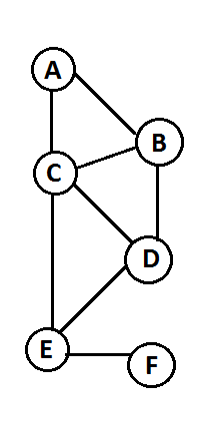
\includegraphics[width=0.9\columnwidth]{img/graph1.png}
	\caption{Beispiel für die Darstellung eines Graphen \parencite[vgl.]{Kleinberg-2009-oz}}
	\label{fig:graph1}
	\end{center}
\end{dsafigure}

Innerhalb der Struktur des Graphs kann es Besonderheiten, wie z.B.\ Komponenten geben.
Das bedeutet, es gibt einzelne Netzwerke, welche nicht über einen Pfad mit jedem anderen Knoten im Graph verbunden sind.

\begin{dsafigure}
	\begin{center}
	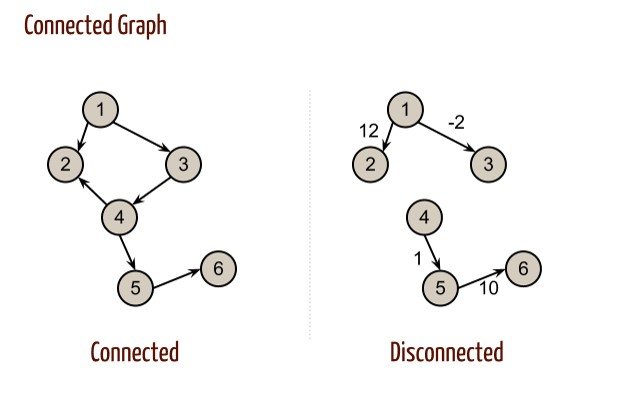
\includegraphics[width=0.9\columnwidth]{img/Graph-Connected.jpg}
	\caption{Beispiel für unverbundene Graphen \parencite[vgl.]{Kleinberg-2009-oz}}
	\label{fig:graph-connected}
	\end{center}
\end{dsafigure}


\subsubsection{Schlussfolgerungen aus der Netzwerktheorie}

Aus dieser Ausgangssituation kann man je nach Betrachtungsweise verschiedene Schlussfolgerungen ziehen.
Beispielsweise kann man den Informationsfluss in Netzwerken analysieren.


\paragraph{Kaskaden und Cluster}

Mithilfe von Graphen ist es möglich, die Ausbreitung von Ideen oder Technologien innerhalb eines Netzwerks zu beschreiben.
Hierbei geht man von einer bestimmten Anzahl von Subjekten (also Knoten) aus, die diese Neuerung benutzen.
Ihre Nachbarn werden dann nacheinander entscheiden, ob sie diese übernehmen möchten oder nicht.
Die Ausbreitung von Technologien sei etwa abhängig vom inhärenten Wert der Neuerung \emph{und} der Nutzung durch relevante Andere.
Eine Käuferin mag sich etwa für ein Faxgerät entscheiden, wenn genügend ihrer Bekannten ebenfalls ein Faxgerät besitzen.
Nur dann kann sie die Neuerung sinnvoll nutzen.
Dies wird entschieden durch einen \emph{Grenzwert} (Threshold), der angibt, welcher Anteil von Nachbarn die Neuerung mindestens benutzen müssen, damit man diese auch übernimmt.
Dementsprechend findet eine Ausbreitung durch das Netzwerk, eine Kaskade, statt.

Diese wird in einigen Fällen gestoppt, endet also, ohne das gesamte Netzwerk übernommen zu haben.
Liegt der Grenzwert für eine Neuerung beispielsweise bei $0,4$, müssen also mindestens $2/5$ der Nachbarn von Knoten $X$ diese Neuerung benutzen, damit sie übernommen wird.
Wenn $X$ aber vier Nachbarn hat, von denen nur einer die Neuerung hat, ist eine Veränderung für $X$ nicht attraktiv genug.
Gehen wir aber davon aus, dass alle anderen Nachbarn von \emph{X} nur untereinander verbunden sind und einen eigenen Abschnitt des Netzwerks bilden und somit nur über \emph{X} ein Pfad zu anderen besteht, gibt es keine Möglichkeit für \emph{X}, den Grenzwert zu erreichen, es kommt zum Ausbreitungsstopp ––– die Kaskade \emph{terminiert}.
Diese Abschnitte innerhalb von Netzwerken bezeichnet man als \emph{Cluster}, also Bereiche des Netzwerks mit eng untereinander verbundenen Knoten, die allerdings nur wenige Verbindungen zu Knoten außerhalb des Clusters haben.
An den Grenzen dieser Cluster terminiert die Kaskade einer Neuerung, da der Treshold für Außenstehende nicht erfüllt werden kann.
Eine eng verbundene Gruppe innerhalb eines Netzwerks sorgt also für eine \emph{Isolation} einer Neuerung von anderen Teilen des Netzwerks.
Besonders deutlich wird dies beispielsweise beim Sprachgebrauch und Vokabular innerhalb der SchülerAkademie;
So gehören Begriffe wie ``KüA'' (kursübergreifende Musik) oder ``AKL'' (Akademie- und Kursleitende) in der DSA zum normalen Sprachgebrauch und sind bei allen Teilnehmenden etabliert.
Sie werden sich allerdings kaum darüber hinaus in den Wortschatz ausbreiten, da die DSA einen eigenen, von anderen Bereichen isolierten Kontext darstellt.
Die Netzwerktheorie macht deutlich, weshalb bestimmte gemeinsam geteilte Angewohnheiten oder Neuerungen sich nur in einem bestimmten Cluster etablieren und somit große Netzwerke in kleinere Abschnitte unterteilen, die wiederum in ihren Eigenschaften mehr oder weniger unabhängig und isoliert voneinander bestehen.
Diese relative Isolation kann in bestimmten Fällen sowohl einen Vorteil der Mitglieder innerhalb der Gruppe als auch eine Abgrenzung von Außenstehenden zur Folge haben, da diese keine Möglichkeit haben, Neuerungen der Gruppe zu übernehmen.


\paragraph{Didaktische Bezüge zum Inklusiven Unterricht nach Zimpel}

Eine Anwendung in der Pädagogik bietet \textcite{Zimpel2012}, der in seinem Text als ein zentrales Problem des Lehrens in der Schule die Heterogenität in einer Lerngruppe beschreibt, durch die ein Konflikt zwischen der Möglichkeit einer individuellen Förderung und dem Ziel eines gemeinsamen Lernens, das jeden Schüler in gleicher Weise berücksichtigt, entsteht.
Die Lehrenden müssen sich also der Frage stellen, welches der beiden Ziele, Individualität oder Gemeinschaft, auf Kosten des anderen stärker verfolgt werden soll.
\citeauthor{Zimpel2012} stellt drei Möglichkeiten vor:

\begin{enumerate}
	\item Ein Prinzip, bei dem die Individualität des Einzelnen in den Vordergrund gestellt wird, ist das \emph{Matthäusprinzip}.
	Sein Grundsatz sagt aus: ``Wer viel hat, dem wird viel gegeben; wer wenig hat, dem wird genommen.'' \parencite[105]{Zimpel2012}.
	Man kann es damit erklären, dass Menschen mit \emph{mehr} (zum Beispiel Begabung oder Geld) bessere Voraussetzungen haben und automatisch leichter \emph{noch mehr} erreichen als andere mit  \emph{weniger}, wodurch sich die Unterschiede verstärken.
	Oft findet dies auch bewusst in Form von gezielter Förderung und speziellen Programmen für leistungsstarke Schüler wie beispielsweise der DSA statt.
	Diese leistungsstarken Schüler bilden dann in der Gesamtschülerschaft ein eigenes Cluster, durch das sie sich von den anderen leistungsschwächeren Schülern abgrenzen.
	Sie bekommen so Zugang zu speziellen Inhalten, Methoden oder auch wichtigen Kontakten und Möglichkeiten, von denen sie untereinander profitieren, zu denen schwächere Schüler aber keinen Zugang finden können.
	Zum einen entstehen dadurch größere gesellschaftliche und schulische Disparitäten, andererseits bietet sich aufgrund der verschiedenen Fähigkeitsstufen eine Wettbewerbssituation, die als Motivation für schwächere dienen kann.

	\item \emph{Das Normalisierungsprinzip} kann als Gegenstück des Matthäusprinzips betrachtet werden: ``Wer wenig hat, bekommt. Wer viel hat, gibt.'' \parencite[12]{Zimpel2012}.
	Durch verschiedene Maßnahmen wird hier ein Ausgleich angestrebt.
	Die Anzahl der Schüler, die dem Mittelmaß zugeordnet werden können, steigen demnach an.
	Extreme Abweichungen nehmen entsprechend ab.
	Besonders in der Sonderpädagogik wird dieses System häufig angewendet, um benachteiligten Schülern gleiche Chancen einzuräumen.
	Als Netzwerk dargestellt, gäbe es beim Normalisierungsprinzip keine Cluster oder Abgrenzungen, da jeder Schwache mit starken Schülern in Kontakt steht.
	Das Ideal dieses Prinzips wäre eine Lerngruppe, in der ein homogener Bildungsstandard herrscht.
	In der Netzwerktheorie stößt das Prinzip allerdings schon an seine Grenzen, wenn man Personen am Rand des Netzwerks betrachtet, die zwangsläufig weniger Kontakte als andere haben.

	\item Da diese beiden Prinzipien, werden sie als einziges und vollständig angewendet, gravierende Nachteile mit sich bringen, stellt \citeauthor{Zimpel2012} eine dritte Möglichkeit vor, wie die beschriebenen Probleme didaktisch gelöst werden könnten: den \emph{Hyperzyklus}.
	Dieses Prinzip erläutert, wie Integration als Balance zwischen Anerkennung von Individualität und Gleichwertigkeit aller Schüler gelingen kann.
	Der didaktische Hyperzyklus beruht darauf, dass sich alle Schüler als hilfreich für andere erleben können.
	So entsteht ein rekursives, zirkuläres System von gegenseitiger Hilfestellung (Rot hilft Gelb, Gelb hilft Grün, Grün hilft Rot, etc.).
	Es entsteht ein ``Fluss des Gebens und Nehmens'' \parencite[125]{Zimpel2012}, bei dem, trotz der unterschiedlichen Voraussetzungen der Schüler, alle in den Lernprozess eingebunden werden konnten.

	Auch beim Hyperzyklus gibt es dementsprechend keine Clustergrenzen und somit keine Abgrenzung zwischen Schülern verschiedener Leistungsstärken.
	Das Prinzip kategorisiert nicht zwangsläufig in stark oder schwach, sondern differenziert den Leistungsbegriff und berücksichtigt viele verschiedene Fähigkeiten und Begabungen.
	Somit kann jeder Schüler als Hilfe dienen und Hilfe empfangen.
\end{enumerate}
%MH TODO tatsächlich ist die oben genannte Anwendung von Netzwerktheorie auf Zimpel noch nicht überzeugend; langfristig müsste man diesen Teil nochmal aufrollen. Der Zusammenhang zwischen Zimpel und Netzwerktheorie ergibt sich – wenn überhaupt – nur über die Power Law Dynamiken von *manchen* Netzwerkeffekten, also die skalenfreie Verteilung ihrer Graphen.


\paragraph{Power Law}

Wie sich bereits mithilfe der Graphen- und Netzwerktheorie erklären ließ, hat jeder Mensch innerhalb eines Netzwerks einen bestimmten, klar definierten Bekanntenkreis aller mit ihm verbundenen Nachbarn.
Dieser ist in der Realität in den meisten Fällen zahlenmäßig überschaubar, allerdings gibt es Ausnahmen von prominenten Personen, deren Bekanntheit über ihren direkten Bekanntenkreis hinausgeht.
In manchen Fällen (z.B.\ bei Barack Obama) kommt es sogar zu globaler Bekanntheit.
Das selbe Phänomen erkennen wir bei anderen Medien, die Popularität erlangen können wie Musik, Bücher, etc.
Daraus ergibt sich für Kleinberg die grundlegende Fragestellung:
Wenn jeder Mensch einen messbaren Bekanntheitsgrad $k$ besitzt, wie lässt sich die Verteilung der verschiedenen $k$ in der Gesamtbevölkerung als Funktion modellieren?
Einen naheliegenden Ansatz stellt die Normalverteilung dar, welche bei vielen Phänomenen in der Natur Anwendung findet.
Hierbei scharen sich die Anteile um einen Mittelwert und sinken für größere und kleinere $k$ exponentiell ab.

Ein anderer Ansatz ist das \emph{Power Law}.
Kleinberg bringt hierbei das Beispiel von Internetseiten, modelliert man für diese die Verteilung der Bekanntheiten, ergibt sich eine hyperbelförmige Kurve mit der Funktion $1/ k^2 $.
Wertet man die Daten mehrerer Verteilungen aus, so zeigt sich, dass das Power Law im Großteil der Fälle überwiegt, wenn auch die Funktionen sich in ihren Parametern leicht unterscheiden (So zum Beispiel $1/ k^3$ bei Romanen).
Allerdings gilt für alle die allgemeine Gleichung des Power Law:
$f(k) = a/(k^c)$.
Der Vorteil dieses Modells und der Unterschied zur Normalverteilung besteht im Verhalten des Graphen für große $k$:
Während die Anteile bei exponentieller Abnahme mit steigendem $k$ gegen Null streben, sinkt die Kurve beim Power Law deutlich langsamer.
Das bedeutet, dass die Werte für hohe $k$ deutlich größer sind und dass auch höhere Werte für $k$ erreicht werden können.
In der Praxis erklärt dieses Modell damit das Zustandekommen von Prominenz und Berühmtheit sowie das Auftreten in extremer Ausprägung, bei der einzelne Menschen fast uneingeschränkte globale Popularität erlangen können.

	%!TEX root=../Emile.tex

\subsection[Spieltheorie]{Spieltheorie: Was ist deine Strategie?}

\epigraph{
	``Gentlemen, Adam Smith needs revision.''\\*
	\emph{Fiktionaler John Nash im Kinofilm ``A Beautiful Mind'' (2001)}
}

Die \emph{Spieltheorie} modelliert menschliche Interaktion in Form von Spielen, dessen \emph{Spielausgänge} von den gewählten \emph{Spielstrategien} abhängen und in Form einer Auszahlungsmatrix analysiert und veranschaulicht werden können \parencite[vgl.][153-274]{Kleinberg-2009-oz}.

\begin{quote}
	``Game theory is concerned with situations in which decision-makers interact with one another, and in which the happiness of each participant with the outcome depends not just on his or her own decisions but on the decisions made by everyone.''\\*
	\textcite[vgl.][156]{Kleinberg-2009-oz}
\end{quote}

Bei einem \emph{Spiel} handelt es sich um eine Entscheidungsfindung von Spielern, in der alle Beteiligten wechselseitig von den Entscheidungen der anderen abhängig sind und stets nach Eigeninteresse handeln.
Ein gängiges Beispiel für ein Spiel der Spieltheorie liefert das \emph{Gefangenendilemma}.

\begin{dsafigure}
	\begin{center}
	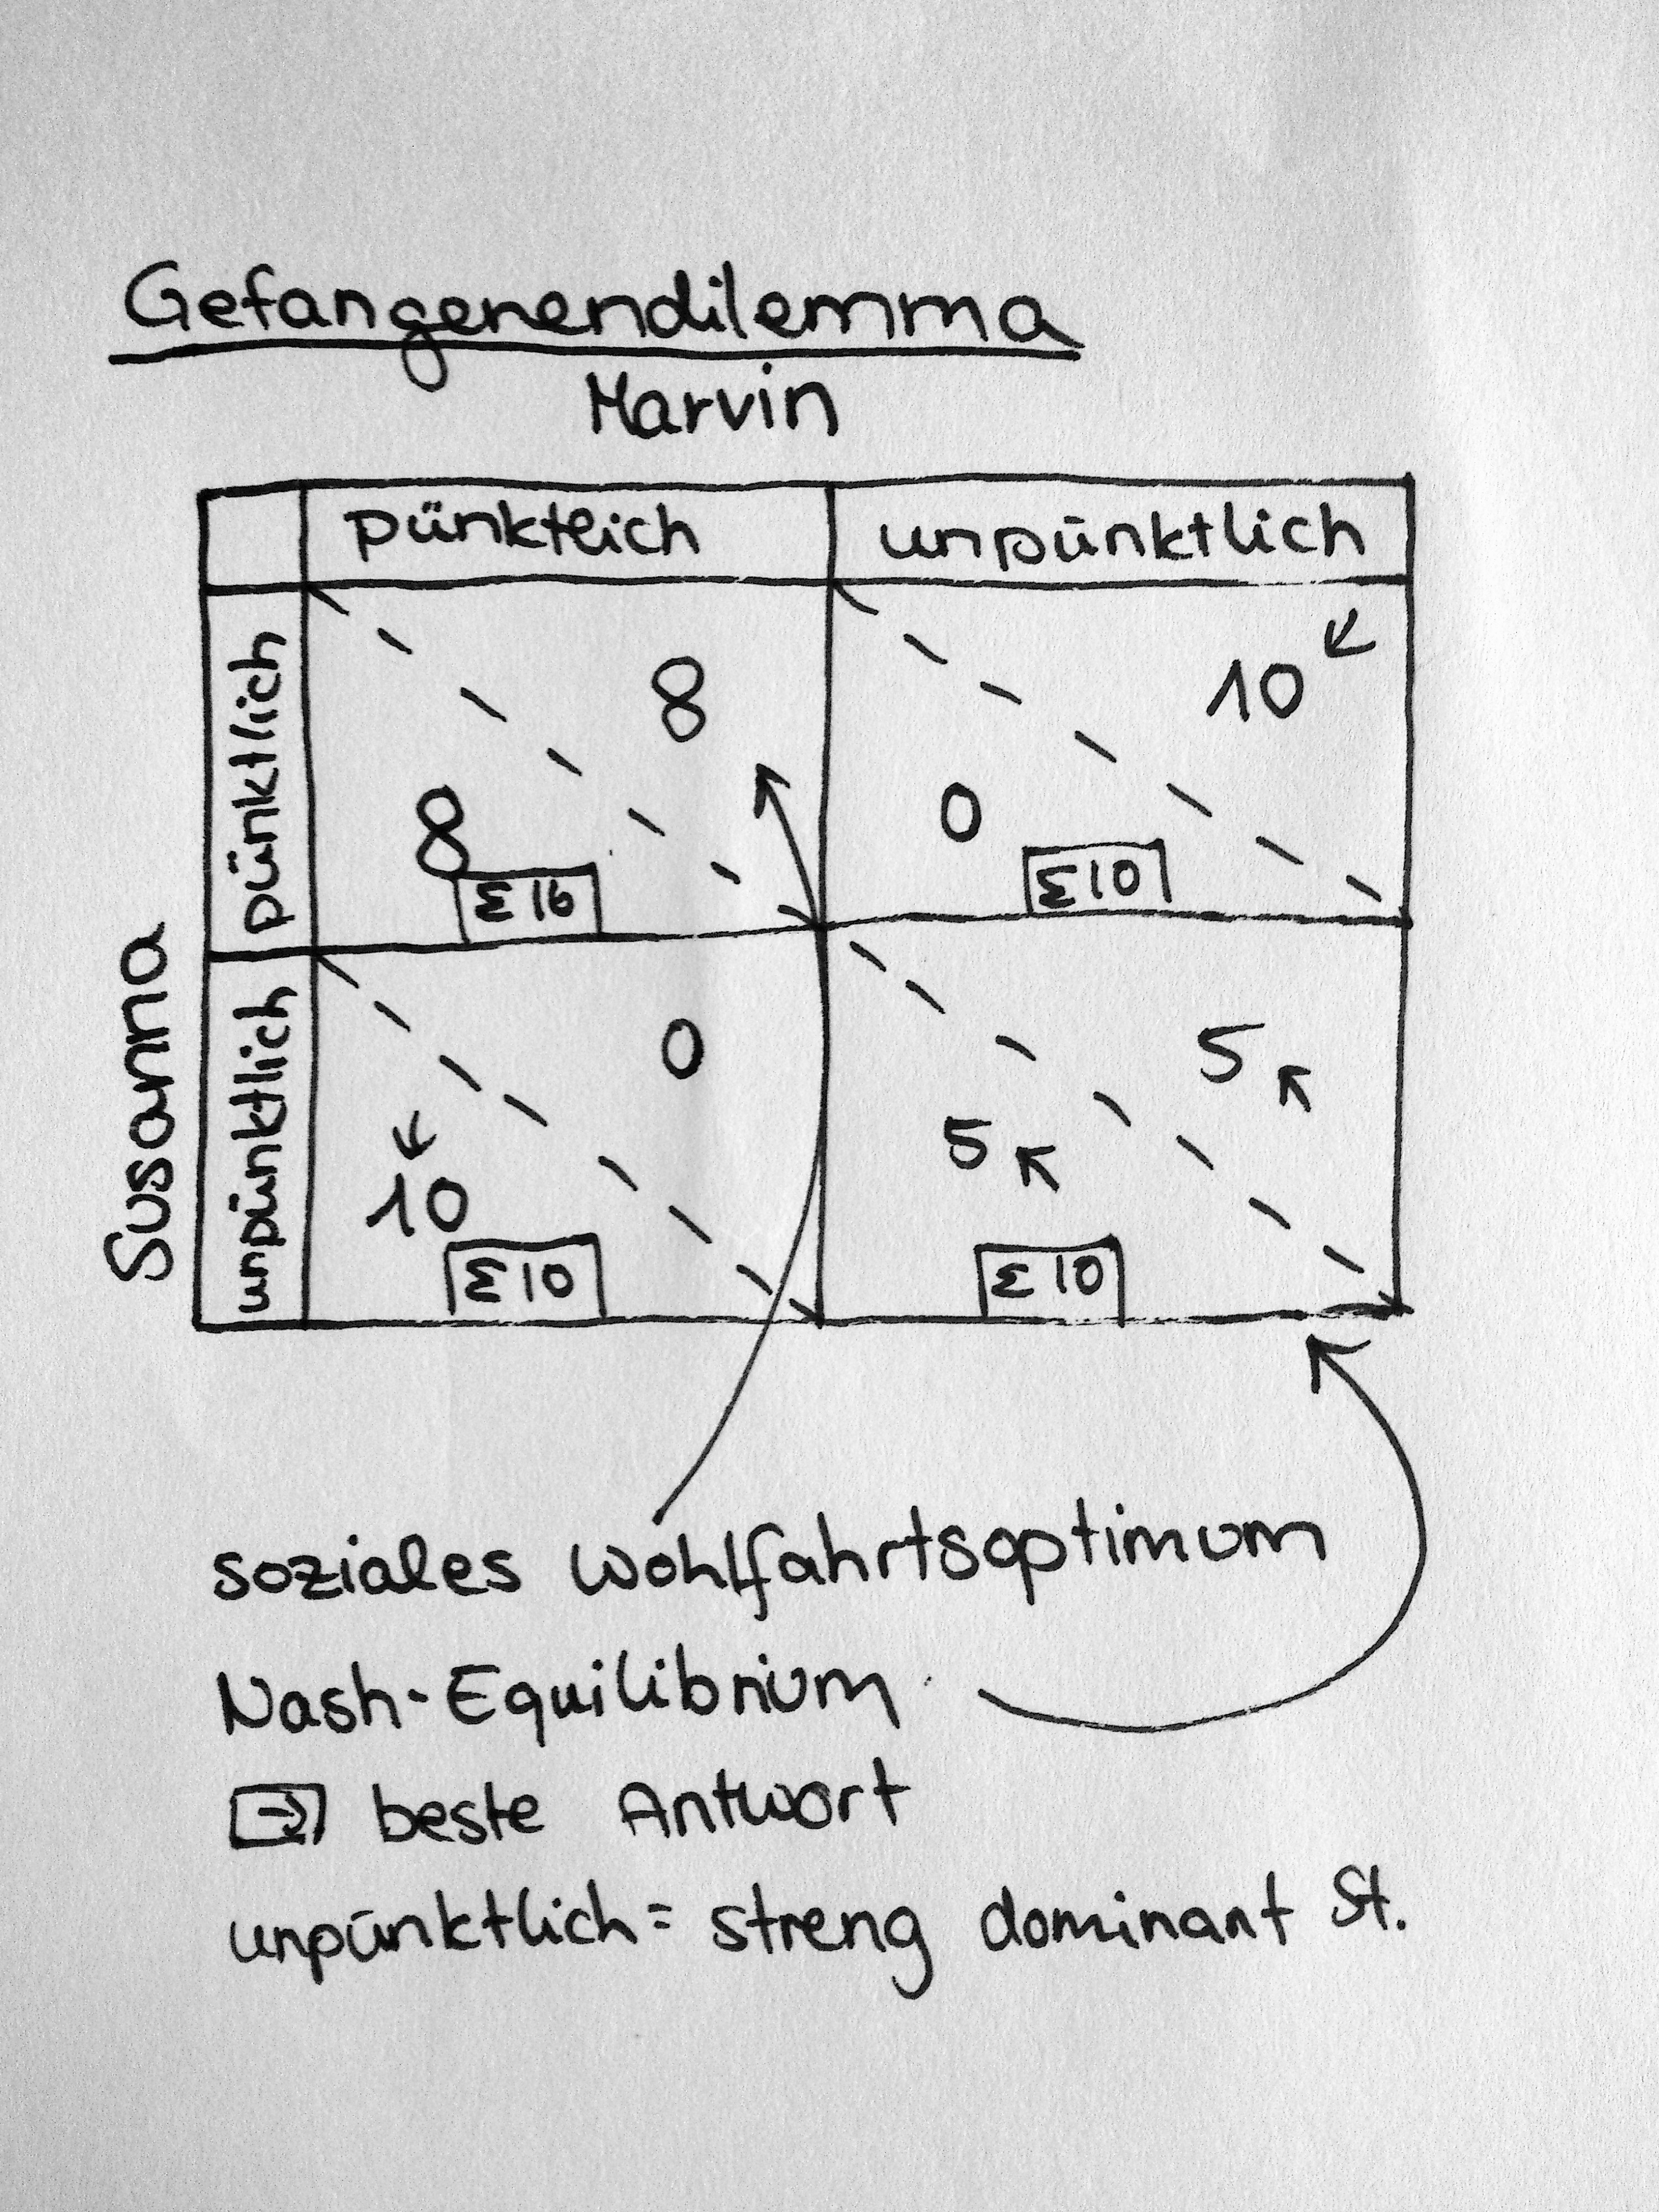
\includegraphics[width=0.9\columnwidth]{img/gefangendilemma.jpg}
	\caption{Beispiel für ein Gefangenendilemma nach \cite{Kleinberg-2009-oz}}
	\label{fig:gefangenendilemma}
	\end{center}
\end{dsafigure}

Die Abbildung oben stellt eine Auszahlungsmatrix dar.
Hier werden die Spielstrategien der Spieler dargestellt und die Summenanzahlen der Zellen in den jeweiligen Entscheidungen.
Verdeutlicht wird hier auch die wechselseitige Abhängigkeit beider Spieler: Wenn sich der Spieler $A$ (Marvin) für eine Spielstrategie entscheidet, so betrifft das auch Spielerin $B$ ()Susanna) und die Auszahlung an beide Spieler.

Das Gefangendilemma ist in mehrer Hinsicht ein Sonderfall, der sich in eine allgemeine Typologie von Spielen einsortieren lässt.

\begin{enumerate}
	\item Zum einem kann es \emph{Nullsummenspiele} geben.
	Dabei haben alle Spielausgänge die gleiche Summen.
	Es gibt lediglich Verteilungseffekte.
	\item Zum anderen kann es \emph{Positivsummenspiele} (wie oben dargestellt) geben.
	In einem Positivsummenspiel haben die Zellen unterschiedliche Summen. Unterschiedliche Spielausgänge führen also zu Wohlfahrtsverlusten oder -gewinnen.
	Tatsächliche Kooperation --- also wechselseitig vorteilhafte Zusammenarbeit --- ist also nur bei Positivsummenspiel gegeben.
	Demnach geben Nullsummenspiele keine Aussage über menschliche Kooperation, da die Summenanzahl bei jedem Spielausgang gleich bleibt.
	Innerhalb von Positivsummenspielen kann ferner unterschieden werden zwischen:
	\begin{enumerate}
		\item Spiele \emph{totaler Harmonie}: \emph{Zellen} von Nash-Gleichgewicht und Wohlfahrtsoptimum fallen hier zusammen.
		Das Nash-Gleichgewicht liegt im Wohlfahrtsoptimum.
		Beispielhaft ist für diesen Spielausgang ist der Handel.
		Adam \textcite{Smith-1776-lq} Theorie der Handelsgewinne kann als Spiel totaler Harmonie verstanden werden:
		\begin{quote}
			``Wer sein eigenes Interesse verfolgt, befördert das Wohl der Gesamtgesellschaft häufig wirkungsvoller, als wenn er wirklich beabsichtigt, es zu fördern.
			Ich habe nie erlebt, dass viel Gutes von denen erreicht wurde, die vorgaben, für das öffentliche Wohl zu handeln.''\\*
			\textcite{Smith-1776-lq}
		\end{quote}

		\item Spiele mit \emph{Kooperationsproblemen}: Summenanzahl von Wohlfahrtsoptimum und Nash Gleichgewicht unterscheiden sich.
		Ein Beispiel wäre das der Nationalen CO2-Emissionen.
		Entscheidet sich ein Land dafür, weniger Umweltschutzmaßnahmen zu treffen, so profitiert es davon nur, solange die anderen Ländern nicht die gleiche Strategie wählen.
	\end{enumerate}
\end{enumerate}

Die verschiedenen Spiele lassen sich auch in einem Baumdiagramm darstellen, wie in Abbildung \ref{fig:gefangenendilemma}.

\begin{dsafigure}
	\begin{center}
	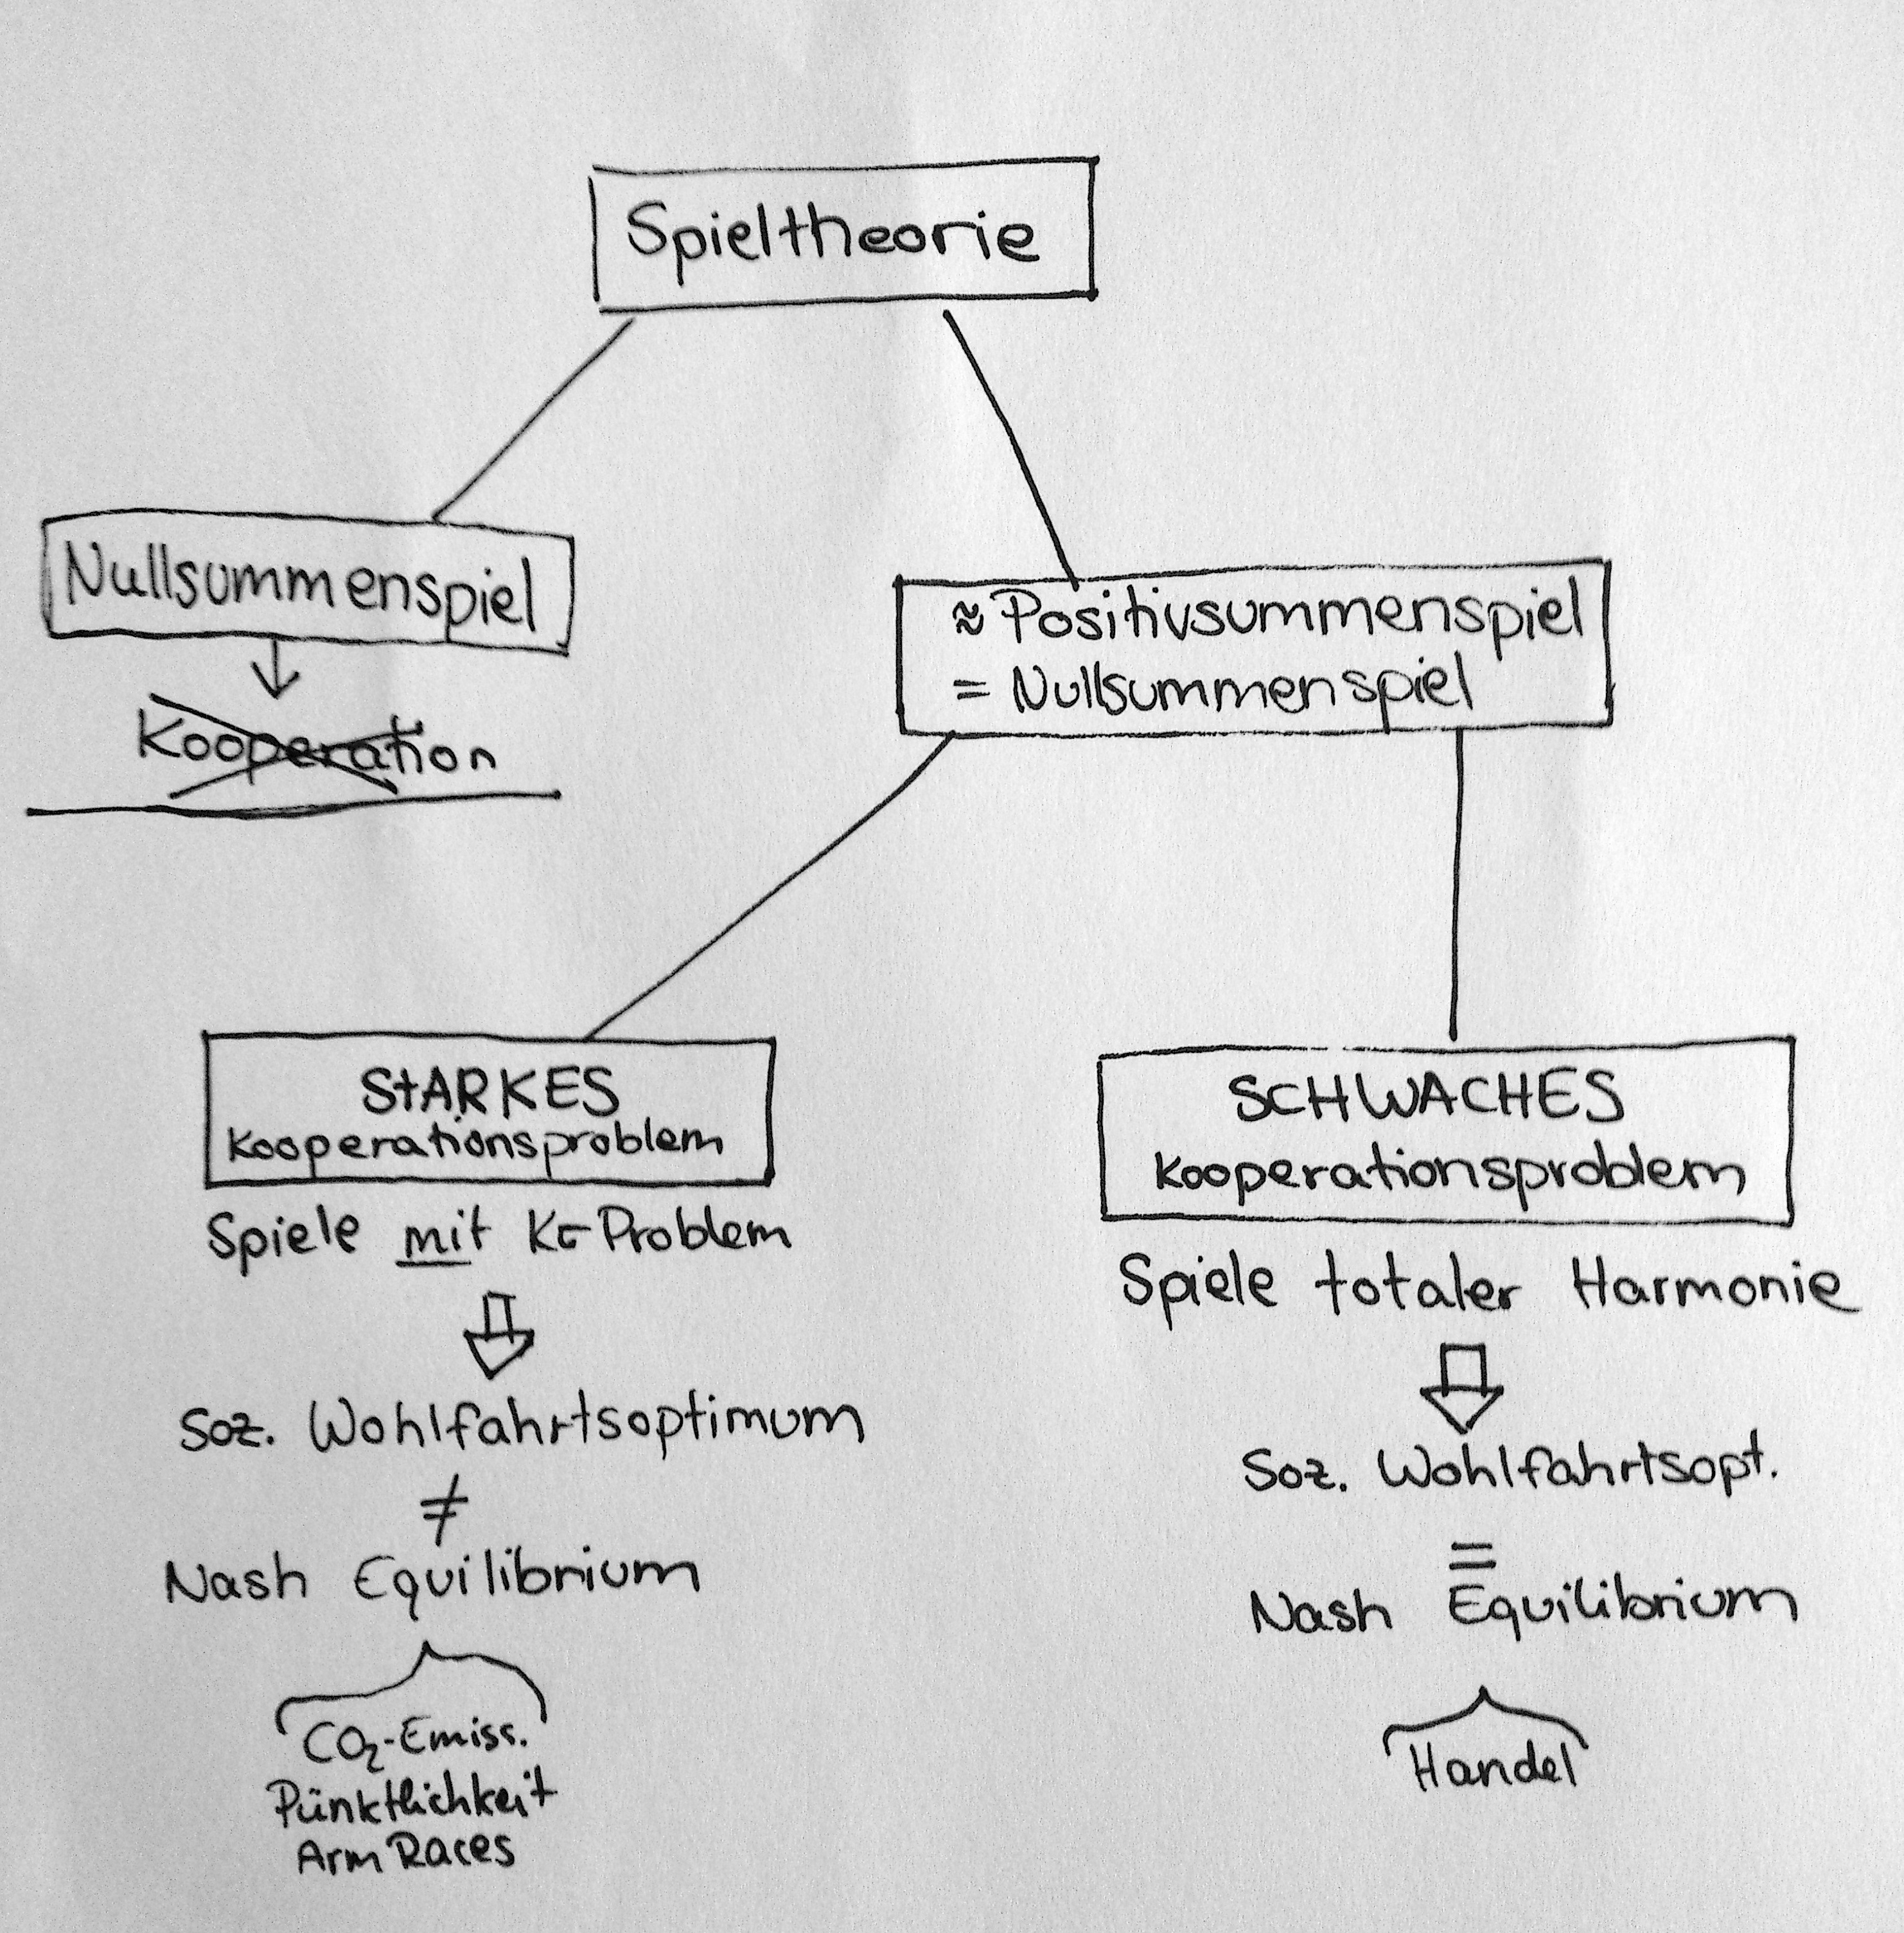
\includegraphics[width=0.9\columnwidth]{img/summenspiele.jpg}
	\caption{Summenspiele nach \cite{Kleinberg-2009-oz}}
	\label{fig:gefangenendilemma}
	\end{center}
\end{dsafigure}


\paragraph{Die Spielstrategien}

Eine Strategie gilt als \emph{beste Antwort}, wenn sie zu der Strategie einer anderen Spielerin am besten passt, d.h. die eigene Auszahlung maximiert.
Hier sind mehrere beste Antworten möglich, wenn die Auszahlungen bei mehreren ``Antwort-Strategien'' gleich sind \parencite[vgl.][153]{Kleinberg-2009-oz}.

Eine Strategie ist \emph{streng dominant}, wenn die Spielerin stets, unabhängig von den Mitspielern, die beste Auszahlung darstellt \parencite[vgl.][164]{Kleinberg-2009-oz}.


\paragraph{Die Spielausgänge}

Ein \emph{Nash-Gleichgewicht} entsteht, wenn die beiden Spieler Strategien gewählt haben, die jeweils die beste Antworten aufeinander sind.
Das \emph{soziale Wohlfahrtsoptimum} ist die Zellenkombination mit der höchsten Summe.

Der Erfolg einer Person im Spiel liegt somit nicht nur in seinen eigenen Entscheidungen, sondern darin welche Spielentscheidungen von allen anderen getroffen werden \parencite[vgl.][156]{Kleinberg-2009-oz}.


\paragraph{Die Axiome der Spieltheorie}

Nach Annahme der Axiome der Spieltheorie entscheidet sich die Spielerin in seinem Handeln stets streng ökonomisch, das heißt, sie verfolgt die Strategie mit dem größtmöglichen Gewinn.
Außerdem wird angenommen, dass jeder den \emph{Spielplan} kennt und somit auch alle Spielstrategien und Mitspieler.
Die letzte Annahme basiert auf der rationalen, individuellen Nutzenmaximierung \parencite[vgl.][159]{Kleinberg-2009-oz}.


\paragraph{Das Gefangenendilemma lösen}

Außer durch den Einfluss eines Gewaltmonopolists oder einer Änderung der Axiome, wie z.B.\ der Annahme des ``Gemeinwohls'' (vgl. \citeauthor{rousseau-1762}), kann das Gefangenendilemma nicht gelöst werden, da alle Spieler nur aus Eigeninteresse handeln.
Dieses Problem wäre durch Tillys Theorie der \emph{Staatsgenese} gelöst, sie stellt hierzu einen Gewaltmonopolisten bereit \parencite{Tilly-1985-aa}.

Adam Smith lag somit mit seiner Annahme, dass die \emph{streng dominante} Spielstrategie stets auch am besten zum Allgemeinwohl beiträgt falsch, da man nicht grundsätzlich von Spielen mit \emph{besten Antworten} ausgehen kann und es dementsprechend, wie aufgezeigt, auch zu Kooperationsproblemen in menschlicher Interaktion kommen kann.


\paragraph{Anwendung der Spieltheorie}

Wie lässt sich die Spieltheorie in den Kurszusammenhang einordnen?
Das Modell der Spieltheorie stellt eine deutlich präzisere Formulierung des \emph{Kooperationsproblems} in der menschlichen Interaktion dar, indem es dieses auf ein mathematisches Modell zurückführt.
Durch diese Vereinfachung steht die Spieltheorie von Kleinberg aber auch in einem starken Kontrast zu dem Menschenbild der anderen Sozialwissenschaftler und Pädagogen, die wir im Kurs besprochen haben.
Kritisch zu hinterfragen ist, ob es sinnvoll ist, menschliche Kooperationsprobleme auf ein mathematisches System zurückzuführen beziehungsweise den Menschen durch Mathematik erklären zu wollen.

\section{Epilog}
	%!TEX root=./Emile.tex
\subsection[Dewey]{Ein Plädoyer für den Fortschritt}

Wie der Romantiker und Republikaner \citeauthor{rousseau-1762}, denkt auch der Philosoph, Sozialwissenschaftler und Pädagoge \citeauthor{Dewey2010} in seinem Werk Demokratie und Schule zusammen.
Vom Skeptiker der Moderne Rousseau unterscheidet ihn aber seine pragmatische Fortschritts-Ethik.
Für \citeauthor{Dewey2010} müssen fortschrittliche Ideen des guten Handelns zwar immer in der  praktischen Erfahrung der Gegenwart (etwa: menschenwürdiges Einkommen) formuliert sein, sie haben aber immer über diese gegenwärtige Praxis hinaus zu deuten, und dürfen keinesfalls \emph{realistisch} einem Status Quo idealisieren.
Es wäre nach \citeauthor{Dewey2010} also fatal, würde man seine ethischen Vorstellungen der gegenwärtigen Realität anpassen.

\paragraph{Theorie des guten Handelns}

Die Theorie des guten Handelns hat eine deontologische Ethik als Grundlage, welche von transzendentalen Pflichten ausgeht.
Sie erschöpft sich also nicht in der Beschreibung ihrer Konsequenzen.

Eine weitere Grundlage der Theorie ist der Konsequentialismus.
Dieser sagt aus, dass das Handeln gut ist, wenn die Ergebnisse gut sind.
Demnach müssen die Konsequenzen aus der jeweiligen Handlung auch gut sein.

Der Pragmatismus bildet hierbei die Synthese zwischen diesen beiden sich widersprechenden Theorien.
Dieser sagt nämlich aus, dass wir eine Ethik inne haben, die durch den Horizont der Praxis definiert ist und deshalb angepasst werden muss.

\paragraph{Deweys gesellschaftliches Ideal}

\citeauthor{Dewey2010} sieht den Fortschritt vom Naturzustand zur Demokratie als einen Suchprozess nach dem Ideal.
Fortschritt kann weiterhin auch durch Angst bewirkt werden.
Zum einen sieht \citeauthor{Dewey2010} Angst als Druckmittel der staatlichen Gewalt, zum anderen aber auch als Motivation, Aufgaben besser auszuführen.
Daraus ist abzuleiten, dass Angst tendenziell nicht als schlecht angesehen wird.
Sie wird allerdings häufig auf falsche Art und Weise institutionalisiert und verliert somit ihren möglicherweise positiven Effekt.
Im Sinne der Motivation kann mit Angst allerdings ein Problem auftreten, wenn z.B. die Arbeiterinnen nicht wissen, warum sie etwas machen, sondern nur in Erwartung von Belohnung bzw. Bestrafung agieren.
Findet eine Mitarbeiterin keine Form von Selbstverwirklichung in ihrem Beruf, so findet sich nach \citeauthor{Dewey2010} legale Sklaverei.
Wie sich an der folgenden Kritik Deweys an Platos Klassengesellschaft erkennen lässt, sind dabei laut \citeauthor{Dewey2010} der Individualismus, die Chancengleichheit und der Meinungsaustausch in einer Demokratie wichtig, damit es in der Gesellschaft die ständige Möglichkeit zur Neuausrichtung und Verbesserung gibt:
``He never got any conception of the indefinite plurality of activities which may characterize an individual [...] ans consequently limited his view to a limited number of \emph{classes}.'' \parencite[95]{Dewey-1916}
``Hence education would soon reach a static limit in each class, for only diversity makes change and progress.'' \parencite[96]{Dewey-1916}

Des Weiteren wird idealerweise die politische Mitwirkung jeder Einzelnen gewährleistet.
Alle müssen gehört werden, denn sie könnten etwas sehen.
Die Gesellschaft darf also nicht in Klassen geteilt werden, zwischen welchen kein Austausch stattfindet und die somit verhindern, dass freie Interaktion zwischen ihren Mitgliedern stattfinden kann.

Hier findet sich ein deutlicher Unterschied zu Rousseau, der in keinster Weise Fortschritt als Ideal betrachtet, sondern stattdessen den Naturzustand des Menschen.

\paragraph{Deweys Erziehungsideal}

\citeauthor{Dewey2010} geht davon aus, dass das Subjekt durch die Erziehung und die Gesellschaft bestimmt wird, denn ``jede Erziehung in einer Gruppe und durch eine Gruppe wirkt sozialisierend'' \parencite[115]{Dewey2010}.
Des Weiteren ist ``die Demokratie [...] mehr als eine Regierungsform, sie ist in erster Linie eine Form des Zusammenlebens, der gemeinsamen und miteinander geteilten Erfahrung'' \parencite[121]{Dewey2010}.
Die Demokratie ist für \citeauthor{Dewey2010} nämlich wichtig für seinen zentralen Erziehungsbegriff.
Diese Demokratie muss allerdings auf einer dynamischen Gesellschaft basieren und als Aufgabe, Projekt oder auch Ziel von allen gesehen weden.
Davon ausgehend lässt sich aus Deweys pädagogischen Theorien schlussfolgern, dass er gar keinen Konflikt zwischen persönlicher Autonomie und inhärenter Gleichwertigkeit sieht.
Beides ist für eine demokratische Erziehung nach Dewey notwendig, und ergänzt sich \parencite[121]{Dewey2010}.

\section{Projekt}
	\section[Projekt]{Projekt}


\subsection[Hayek]{Hayek}


\epigraph{
	``The curious task of economics is to demonstrate to men how little they really know about what they imagine they can design.''
	\emph{Friedrich A. Hayek}
	%MH TODO: add correct reference
}

In der Schule werden Informationen vermittelt, welche Informationen lohnt es sich zu vermittelt?
In der Demokratie müssen wir kollektiv verbindliche Entscheidungen treffen, indem wir Information zusammentragen.
Doch wie sehen diese Informationen aus? Welche Arten von Informationen gibt es?

Wissen ist \citeauthor{hayek-1945} zufolge der Beweggrund wirtschaftlichen Handelns.
In seinem Buch ``The use of knowledge in society'' behandelt er die Frage wie ein wirtschaftliches System aussehen sollte.
Informationen spielen dabei eine große Rolle, da diese für Kollektiventscheidungen unerlässlich sind, um demokratische Entscheidungen fällen zu können.
Dabei betrachtet Hayek das Individuum ontologisch als kleinste Einheit, und fragt davon ausgehend wie ein wirtschaftliches System ausgerichtet sein sollte.
Wissen jedoch ``never exists in concentrated or integrated form, but solely as the dispersed bits of incomplete and frequently contradicitionary knowlegde which all the seperate individuals possess'' \parencite[520]{hayek-1945}.

Nach \citeauthor{hayek-1945} entstehen manche Informationen erst in der konkreten Problemsituation, etwa durch eine Abwägung von verschiedenen Gütern bei gegebenen Preissignalen.
Ein Beispiel aus dem Akademie-Alltag: Oft treffen die Mengen an Kaffee und Tee nicht die tatsächliche Nachfrage und es gibt Engpässe oder Überangebote.
\citeauthor{hayek-1945} wäre vielleicht skeptisch, ob der Chancen jedweder zentraler Planung -- etwa durch die Akademieleitung.
Schließlich würde das eine effektive Abfrage von lokaler Teilnehmerinnen-Information über Kaffee- und Teegeschmack erfordern.
Plausiblerweise würden die Teilnehmerinnen ihre zukünftigen Bedürfnisse ungenau einschätzen oder die Küche würde Nachfragespitzen nicht antizipieren.
Eine katallaktische Lösung im Sinne Hayeks könnte es sein, anstelle des pauschal und subventioniert bereitgestellten Kaffees, Heißgetränke über einen Markt bereit zu stellen.
Möglicherweise hätten dann kaufende Teilnehmerinnen Zugang zu ihren tatsächlich, am Markt bepreisten Bedürfnis an Heißgetränken und die Anbieter hätten Anreize, Informationen über zu erwartende Nachfragespitzen (etwa in der Doku-nacht) einzuholen.

\citeauthor{hayek-1945} schätzt charakteristisch das Preissystem als geeigneter ein um lokale, und kontingente -- also abhängig von Umständen -- Informationen zu sammeln.

Wissen besteht nicht nur aus \emph{scientific knowledge}, das heißt immanentem Faktenwissen.
Wissen entsteht oft auch lokal, also erst in einer gegebenen Situation.
Dies ist das Argument, das \citeauthor{hayek-1945} einer Planwirtschaft entgegenstellt:
Planwirtschaft benötigt eine zentrale Aggregation von Informationen; diese ist aber oft ineffizient oder mangelhaft.

Es ist unwirtschaftlich, Informationen zusammenzutragen, die in einer konkreten Situation jedoch nicht einmal zutreffen.
\citeauthor{hayek-1945} zieht ein freiheitlicheres System der Marktwirtschaft aus Gründen der Effizienz vor.
Hayeks Argument für freiheitlichen Markt besteht in seiner Annahme, dass jeder der Kompetenteste für sich selber sei.

\begin{quote}
	``Every individual [...] posseses unique information of which beneficial use can be made only if the decisions depending on it are left to him or are made with his active cooperation.'' \parencite[521]{Hayek-1945}
\end{quote}

Ähnlich forderte \citeauthor{Dahl-1989-aa} auch nach seiner Annahme der persönliche Autonomie als Grundlage einer Demokratischen Gesellschaft, wenn er formuliert,
``Every adult is the best judge of his or herself interest '' \parencite[100]{Dahl-1989-aa}.

Für \citeauthor{Dahl-1989-aa} ergibt sich daraus eine politische Dimension, die Demokratie, in der jeder, zum Beispiel durch Wahlen für sich selbst entscheiden kann.
\citeauthor{hayek-1945} sieht vor allem die wirtschaftliche Dimension: ``weniger Regierung'' \parencite[527f.]{hayek-1945} und kollektive Entscheidungen, wie zum Beispiel Planwirtschaft, desto besser.
Die Entscheidungsgewalt über ökonomische Handlungen sollte also so oft wie möglich bei den Individuen liegen.

Wenn man versucht, das auf das Schulsystem zu beziehen, könnte man sagen, dass die Idee eines Bildungskanons, einer Informationsvermittlung auf objektiver Basis, skeptisch betrachtet werden sollte, da jede Schülerin die für sie relevanten Inhalte selbst bestimmen kann.

	\subsection{Illich -- Mythos Schule: Vorschläge einer alternativen Gesellschaft}

In ``Deschooling Society'' (1971) hinterfragt \citeauthor{Illich-1971} die Stellung und den gesellschaftlichen Einfluss von Schule.
Er eröffnet dabei neue Perspektiven auf die zentrale Frage unseres Kurses nach Formen menschlichen Zusammenlebens.
Sein Konzept beschränkt sich nicht darauf, das bestehende Schulsystem zu verändern, sondern strebt gleichzeitig gesellschaftliche Umwälzungen an.
\citeauthor{Illich-1971} begreift die Schule als ein Paradigma für die Natur von lebensbestimmenden Institutionen, fordert deren Abschaffung und plädiert für eine Gesellschaft, die sich für freie zwischenmenschliche Interaktion ausspricht.
Das Schulsystem erhalte nach \citeauthor{Illich-1971} die Illusion aufrecht, wir könnten Werte wie Bildung genau bestimmen, analysieren und schließlich messen.

\subsubsection{Kritik an der Institution Schule}

\epigraph{
		``Many students [...] intuitively know what the schools do for them. They school them to confuse process and substance.''}
	{
		\citep[3]{Illich-1971
	}

Weil wir Prozess (z.B. Lehren) und Wert (z.B. Lernerfolg) verwechseln, nehmen wir fälschlicherweise an, das eine würde das andere zwangsläufig bedingen.
Führt mehr Lehren automatisch zu mehr Lernen?
Führt eine größere Polizeipräsenz automatisch zu mehr Sicherheit?
Würde dies zutreffen, könnte man Werte wie Sicherheit und Lernerfolg am Umfang des Prozesses (Polizeipräsenz, Schulanwesenheit) messen.
Den Mythos der messbaren Werte beziehen wir schließlich auch auf unsere ``imaginations, and, indeed, man himself '' \citep[19]{Illich-1971}
Prozess und Wert beginnen einen allgemein verbindlichen Charakter zu entwickeln, weswegen das Wissen darüber an die nächste Generation weitergeben und deren Lernprozess somit ebenfalls kontrollieren werden.
Die Schule lehrt: Je mehr Schule, desto mehr Lernerfolg, weshalb wir zur Schule gehen.

Im Gegensatz dazu schreibt \citeauthor{Illich-1971}:
``Most learning is not the result of instruction: It is rather the result of unhampered participation in a meaningful setting.'' \citep[18]{Illich-1971}.
Aus dieser Überlegung heraus errichtet er ein neues Konzept des Lernens in einer \emph{entschulten Gesellschaft}.

\paragraph*{Lernen ohne Schule}

Für Bildung erachtet \citeauthor{Illich-1971} vier Aspekte als notwendig.
Jeder Mensch bedarf neben dem Kontakt zu anderen Gleichaltrigen auch Vorbilder, von denen er unbewusst lernen kann (Sprechen, Laufen, etc.).
Bei komplexeren Sachverhalten benötigt er professionelle Hilfe sowie den Zugang zu Lernobjekten.
Dies will \citeauthor{Illich-1971} über Netzwerke realisieren.
In einer dieser Netzwerke bekäme ein Kind, das Gitarre spielen lernen \emph, einen Zeitraum, in dem es mit anderen gleichaltrigen Kindern spielen kann, jemanden, der ihn bei Problemen und Schwierigkeiten unterstützen kann und als ein Art Vorbild funktioniert und als letztes eine Gitarre und alle anderen möglichen Werkzeuge, die dazu führen werden, dass das Kind erfolgreich den Lernprozess bewältigt.
Deutlich wird in diesem Beispiel, dass \citeauthor{Illich-1971} von einer hohen Selbstständigkeit des Individuums ausgeht.
In diesem Zusammenhang fordert er auch die Reduzierung der Komplexität unserer Umwelt, sodass sie wieder zugänglich für den Alltagsmenschen wird.
So könnten zum Beispiel Firmen subventioniert werden, die ihre Autos wieder leichter verständlich konzipieren, sodass jeder in der Lage ist, Reparaturen selbst durchzuführen.
So gäbe es auch einen praktischen Grund, der zum Lernen motivieren kann.


\paragraph*{Illichs Entschulung der Gesellschaft als Lösungsansatz für die Organisation des menschlichen Zusammenlebens}

Durch sein Konzept eines selbstbestimmten und selbstorganisierten Lernens können viele der Anforderungen, welche die in der Exposition behandelten Texte an den Prozess des Lernens und an das menschliche Zusammenleben stellen, erfüllt und Widersprüche gelöst werden.
Illich beschreibt konkrete Vorschläge zur Umsetzung seiner ``educational revolution'', die als praktische Anwendung verschiedener theoretischer Ansätze verstanden werden können.

So würde der Konstruktivismus Illichs Auffassung des Lernbegriffes unterstützen.
Nach \citeauthor{siebert-2003} entscheide ``das psychische System, was es verarbeiten kann und will'', je nach dem es als viabel, d.h. bedeutend, von dem Individuum wahrgenommen werden \citep[13]{siebert-2003}.
Jeder hat auch nach \citeauthor{Illich-1971} die Freiheit, eine Gelegenheit zum Lernen wahrzunehmen, oder sich dagegen zu entscheiden.

Damit sich dem Lernenden diese Wahlmöglichkeit eröffnet, benötigt er nach \citeauthor{Illich-1971} Zugang zu den vier oben beschriebenen Ressourcen.
Benner geht ebenfalls von gewissen Umständen, insbesondere Bezugspersonen, aus, die dem Zögling erst selbstbestimmtes Lernen ermöglichen.
Allerdings ``muss Erziehung stets dort an ihr Ende gekommen sein, wo pädagogische Fremdaufforderung zur Selbsttätigkeit in Selbstaufforderung übergehen kann.'' \citep[91]{benner-2012}.
So könnte Benners Begriff der Bildsamkeit und Selbsttätigkeit Illichs Kritik an einem einheitlichen Schulsystem untermauern, welches pädagogischen Zwang auch ohne Bedarf fortführt.
Dennoch hält Benner den \emph{Pädagogen} und die \emph{Aufforderung zur Selbsttätigkeit} für notwendig; \citeauthor{Illich-1971} widerspräche dem.
Aber hier wird auch ein Defizit in Illichs Schreiben deutlich, da er sich nur mit dem gesunden Individuum auseinandersetzt.

Obwohl auch die Gruppierung von Gleichaltrigen nach \citeauthor{Illich-1971} abgeschafft werden soll, findet sein Lernen häufig in sozialen Kontexten statt
Ein Beispiel dafür sind seine \emph{Fertigkeitsbörsen}.
Dieser Vorgang lässt sich sehr gut mit dem Konzept des Hyperzyklus beschreiben, dessen Bedingung ist: ``wer etwas weiß oder kann, teilt es mit den anderen'' \citep[123]{Zimpel2012}, was durch Illichs Vorschläge erfüllt wird.
Dadurch, dass nicht mehr wie vorher ``das Grundrecht auf Mitteilung des eigenen Wissens in das Privileg akademischer Freiheit [verkehrt wird], das nur den in einer Schule Beschäftigten verliehen wird'' \citep[97]{Illich-1971}, ist jeder dazu befähigt, andere an seinem Wissen teilhaben zu lassen, während er wiederum von den Fähigkeiten anderer profitieren kann.

Der Ansatz des sozialen Lernens lässt sich auch auf \citeauthor{Dewey2010}  beziehen.
\citeauthor{Illich-1971} und \citeauthor{Dewey2010}  stellen sich beide gegen einen aktiven Lehrprozess und sehen Lernen eher als eine natürliche Eigenschaft des Menschen.
Auch \citeauthor{Dewey2010}  beschreibt seinen ungezwungenen Erfahrungsaustausch als wichtigste Eigenschaft einer fortschrittlichen Gesellschaft und leitet seinen Wert von der Menge an Interaktion innerhalb und mit einer anderen Gruppe \citep[vgl.][89]{Dewey2010}.

Illichs Glaube an den Menschen außerhalb von sozialen Manipulationen ähnelt oft Rousseau, weshalb auch beide einen sehr skeptischen Blick mit fast verschwörungstheoretischen Charakter auf Gesellschaften als Perversionen von Menschsein werfen.
``I see, therefore, in love, hope, and charity the crowning of the proportional nature of creation in the full, old sense of that term'' (https://www.youtube.com/watch?v=vQLWAafp020, zuletzt geöffnet am 04.09.2014)
Rousseau schreibt: ``In der natürlichen Ordnung sind die Menschen alle einander gleich. Ihr gemeinsamer Beruf ist: Mensch zu sein.'' \citep[50]{rousseau-1762}
Beide kritisieren die Identifikation durch Berufe und Rollenbilder, romantisieren den vormodernen Menschen und plädieren für eine unabhängige Erziehung.
Kooperations- und Verständigungsprobleme finden bei beiden wenig Beachtung.
Daraus ergibt sich ein optimistisches Bild einer Gesellschaft ohne Standards und jeglichen Verpflichtungen.


\paragraph*{Gleichwertigkeit und Autonomie nach Illich}

Ein zentraler Punkt, den \citeauthor{Illich-1971} an Schule kritisiert, ist deren Recht zur Bewertung der Schüler durch Zertifikate, die auch in der gegenwärtigen Gesellschaft als einzig legitime Qualifikationen betrachtet werden.
Die Folgen dieser Macht über Bildungswege Einzelner sind weitreichend, was \citeauthor{Illich-1971} mit dem Satz ``School initiates young people into a world where everything can be measured, including their imaginations, and, indeed, man himself.''  \citep[19]{Illich-1971}, veranschaulicht.
Schule produziert, indem sie alles als messbar ansieht, Ungleichheit.
Das impliziert die unterschiedliche Wertigkeit von Menschen und führt somit dazu, dass Schüler nicht nur als ungleich betrachtet werden, sondern auch sich selber als unterschiedlich wertvoll ansehen.
\citeauthor{Illich-1971} schlägt nun vor, das Messen von Fähigkeiten im Bezug auf den Zugang zu Bildungsmöglichkeiten ganz abzuschaffen.
So entsteht ein Menschenbild, dass von der Gleichwertigkeit aller ausgeht, während die beschriebenen Freiheiten und Wahlmöglichkeiten ein Maximum an persönlicher Autonomie ermöglichen.

	\subsection[Habermas]{Habermas: Kommunikatives Handeln}

\epigraph{
	``Reaching understanding is the inherent telos of human speech.''
	\emph{Jürgen Habermas}
}

% Dass Schule und Demokratie eng mit Kooperation und Kommunikation verbunden sind, wurde bereits in den vorangegangenen Abschnitten deutlich (vgl. \citeauthor{Kleinberg-2009-oz} und \citeauthor{mead-1934en}).
% Intersubjektivität ist sowohl bei \citeauthor{Kleinberg-2009-oz} als auch bei \citeauthor{mead-1934en} gegeben:
% Nach Meads symbolischem Interaktionismus entsteht die Identität immer im Kontakt mit anderen Individuen.
% Kleinbergs Kooperationslose Spiele enden aber nicht notwendigerweise im sozialen Optimum.

Jürgen Habermas \citeauthor{Habermas-1998-aa} postuliert in seinem 1998 erschienen Text ``On the Pragmatics of Communication'' einen Telos menschlichen Handelns und menschlicher Sprache und unterscheidet zwischen verschiedenen Handlungsformen.

\begin{dsafigure}
	\begin{center}
	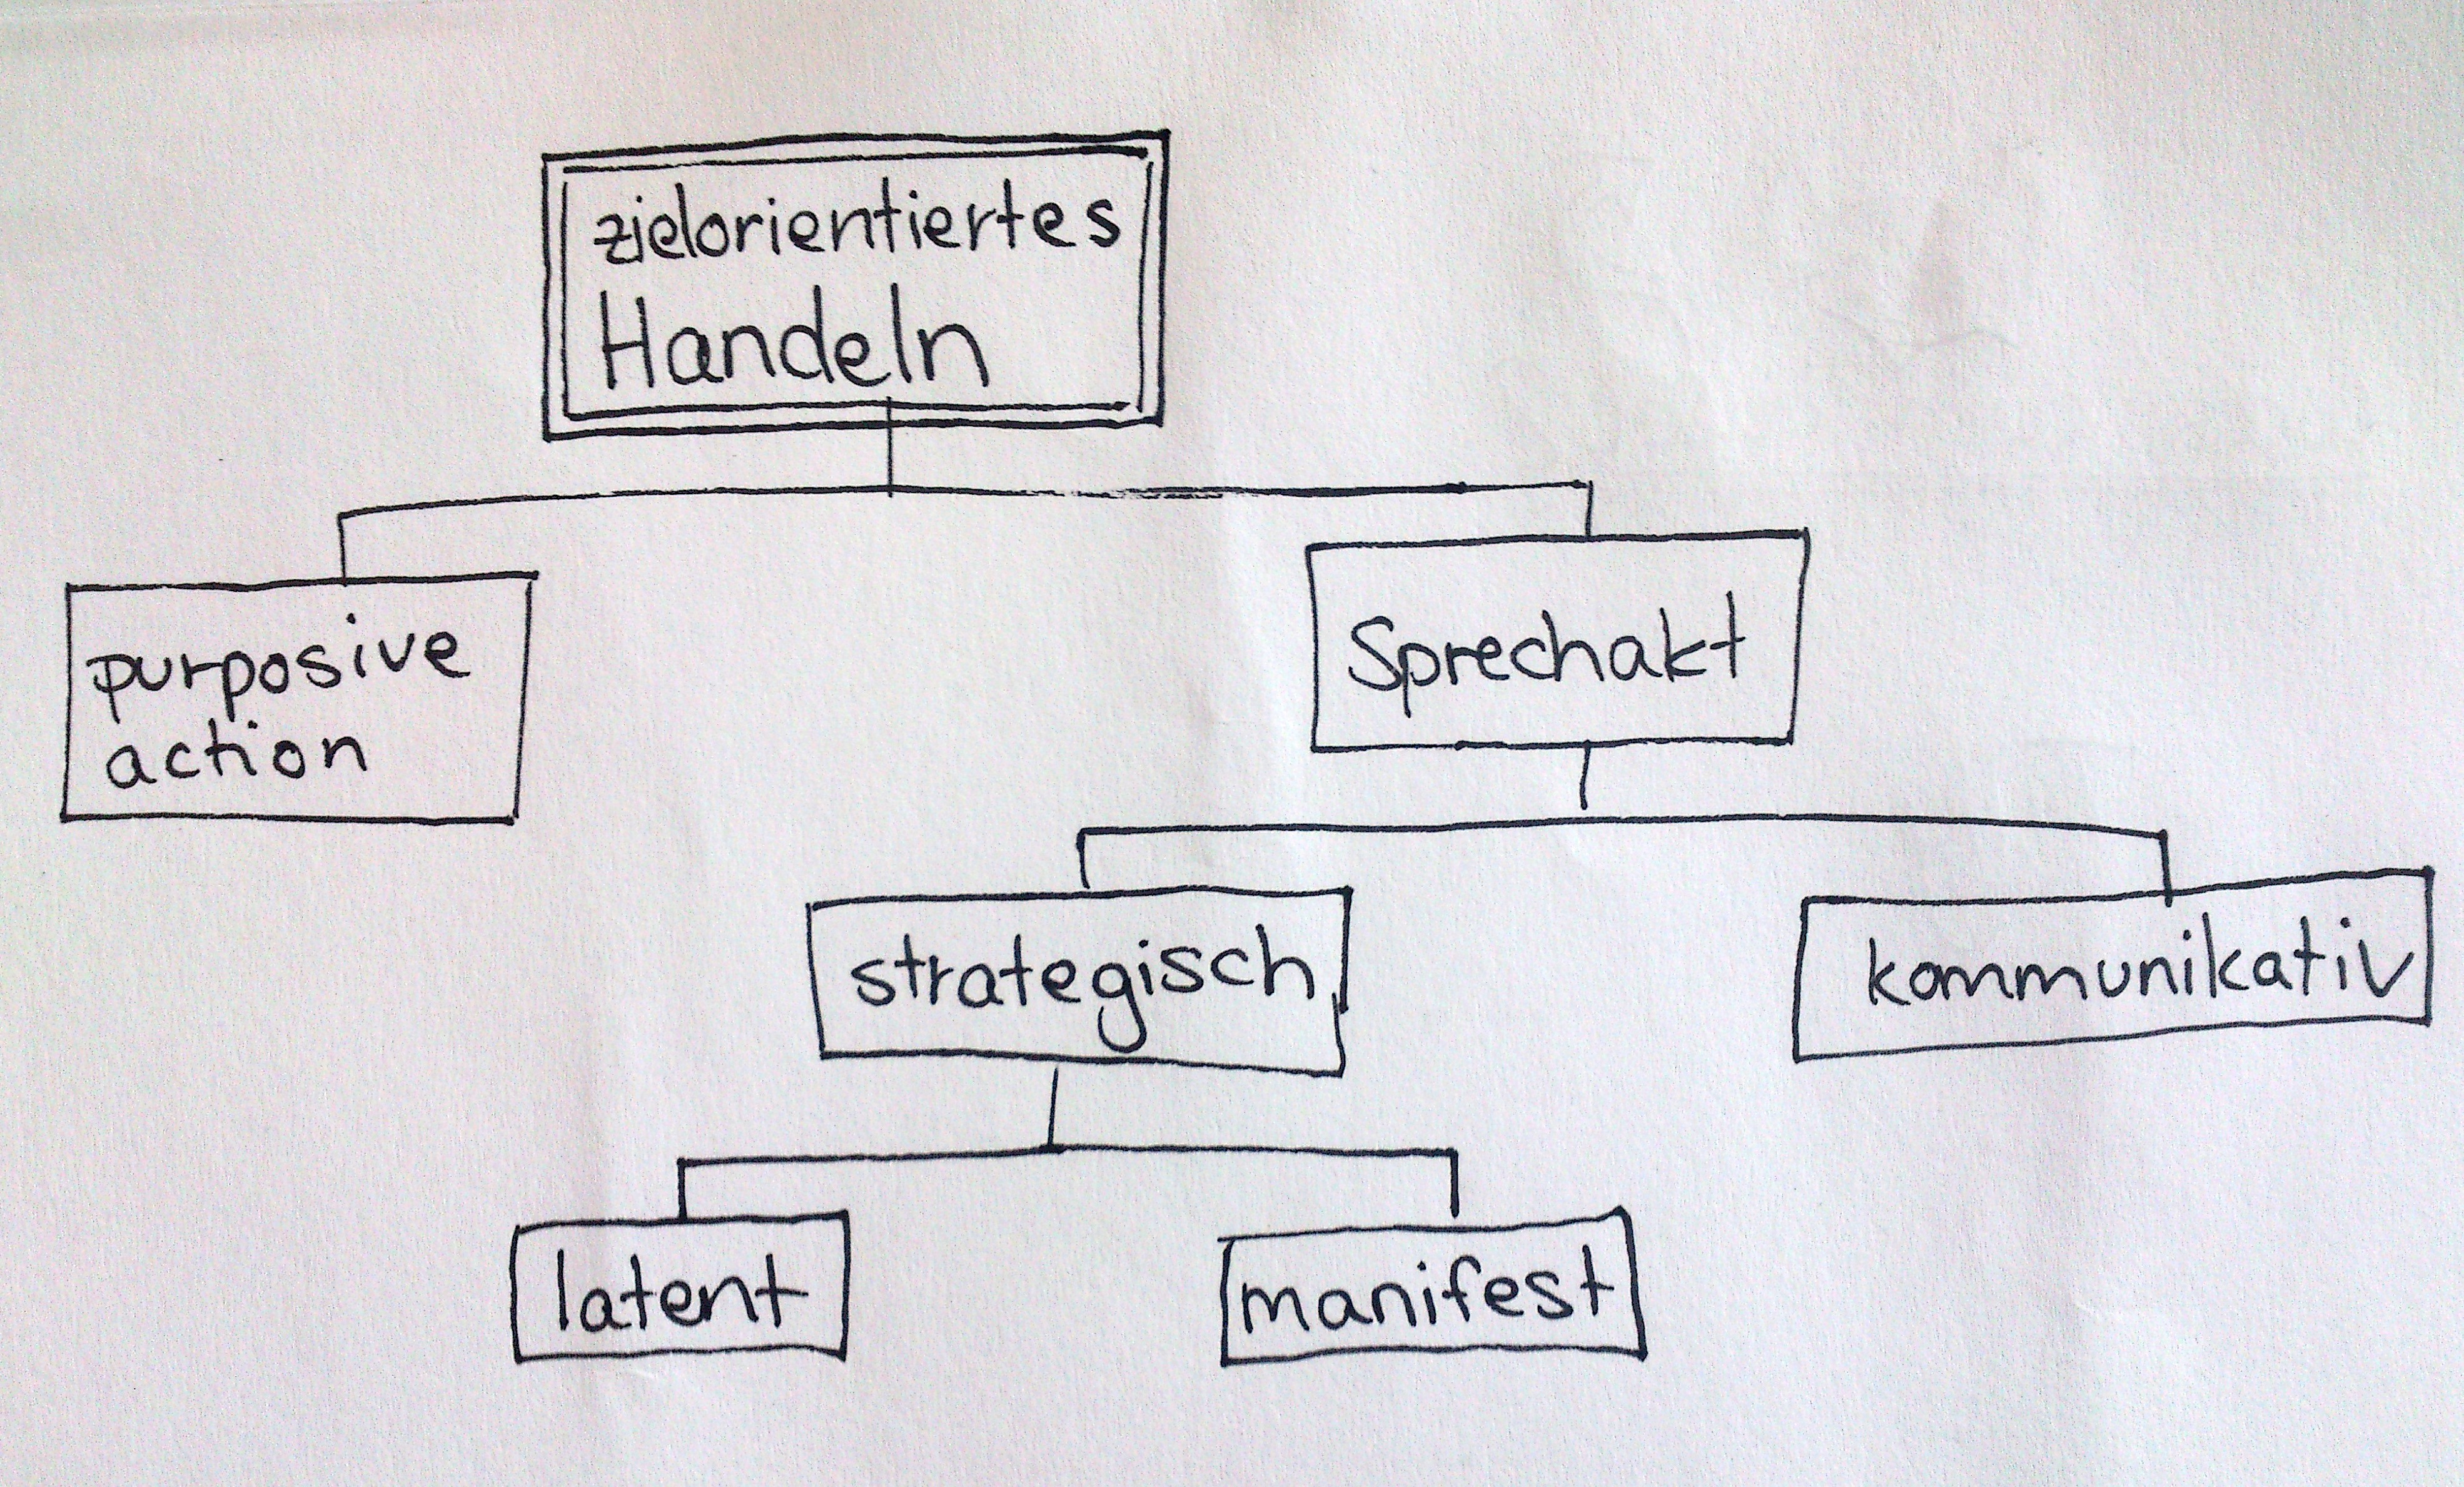
\includegraphics[width=0.9\columnwidth]{img/Habermas_Baumuebersicht.jpg}
	\caption{Handlungsformen nach \cite{Habermas-1998-aa}}
	\label{fig:handlungsformen}
	\end{center}
\end{dsafigure}

Dabei differenziert er zunächst zwischen Handlungen an Objekten in der fassbaren Realität und Handlungen in der sozialen Welt, also Sprechakten, die sich insbesondere in ihren Zielen unterscheiden.

Während die Ziele der Handlungen am Objekt laut \citeauthor{Habermas-1998-aa} kausal herbeigeführt werden können und die Mittel unabhängig vom Zweck stehen, können die Ziele eines Sprechaktes nicht unter diesen Kategorien zusammengefasst werden.
Denn der Sprechakt enthält, im Gegensatz zum Handeln am Objekt, ein sogenanntes illokutives Element, das dem Gesprächspartner die dem Sprechakt zugrundeliegende Absicht des Handelnden offenbart.
Einmal ist deshalb die Annahme der Kausalität unmöglich, denn das Ziel der Verständigung erfordert die Kooperation mit einer zweiten Person und kann damit nicht den selben innerweltlichen Status haben, wie eine Handlung am Objekt.
Außerdem ist auch die Trennung von Mittel und Zweck in der Sprache nicht möglich:

\begin{quote}
	``the medium of natural language and the telos of reaching understanding interpret one another reciprocally, one cannot be explained without recourse to the other.''
	\parencite[218]{Habermas-1998-aa}
\end{quote}

Wenn Hanna, Assistentin der Akademieleitung, im Plenum beispielsweise darauf hinweist, dass die Hilfe beim Drucken der Akademie-T-Shirt wichtig für das Gelingen des Projekts ist, muss sie, um eben diese Verständigung zu erreichen auf Sprache zurückgreifen, welche wiederum einen Verständigungs-Telos impliziert.
Führen wir diesen Gedanken weiter, geraten wir schnell in einen Kreislauf, der die Rekursivität zwischen Sprache und dem Ziel der Verständigung deutlich macht.

Das Telos der illokutiven Verständigung als universelles Ziel menschlicher Sprache steht für \citeauthor{Habermas-1998-aa} teleologisch fest und ist der Ausgangspunkt seiner an die des amerikanischen Philosophen John Rogers Searle und seines britischen Kollegen John Langshaw Austin angelehnten Sprechakttheorie.

Grundsätzlich geht \citeauthor{Habermas-1998-aa}, wie Searle und Austin, davon aus, dass mit jedem Sprechakt automatisch ein Gültigkeitsanspruch auf das Gesagte erhoben wird.
Er grenzt sich allerdings von deren Vorstellung ab, die von Sprechakten aufgestellten Gültigkeitsansprüche würden nur aus Aussagenlogik bestehen.
Er sieht diese stattdessen nur als einen Teil der Gültigkeitsansprüche, die an Sprechakte gestellt werden müssen.

Sagt Mihai, Assistent der Akademieleitung, beispielsweise: ``Wir sollten dem Küchenpersonal etwas vorsingen, weil es jeden Tag unser Essen zubereitet'' kann nach \citeauthor{Habermas-1998-aa} zwar sowohl auf die objektive Wahrheit (Bereitet das Küchenpersonal wirklich unser Essen zu?) aber eben auch auf die normative Richtigkeit (Ist Vorsingen eine angemessene Dankesgeste?), die subjektive Authentizität (Ist das Gesagte auch so gemeint oder wird Mihai von Kerstin gezwungen diesen Vorschlag zu machen?) und die sprachliche Verständlichkeit überprüft werden.
Für \citeauthor{Habermas-1998-aa} muss jeder einzelne dieser Gültigkeitsansprüche anfechtbar sein, um kommunikatives Handeln zu ermöglichen.

Generell differenziert er zwischen \emph{strategischem} und \emph{kommunikativem Handeln}, wobei er letzteres für erstrebenswerter hält.
Zwar steht für \citeauthor{Habermas-1998-aa} grundsätzlich hinter jeder Handlung ein ``action plan'', also ein Ziel, allerdings geht er auch davon aus, dass für eine erfolgreiche Kommunikation die Beilegung dieses ``action plans'' nötig ist, um ausschließlich illokutive Ziele zu verfolgen.
Wird dies nicht getan, spricht \citeauthor{Habermas-1998-aa} von strategischem Handeln, welches perlokutive Ziele, in den Vordergrund stellt, also eine bestimmte Wirkung beim Gegenüber erreichen möchte.
Dabei gibt es wiederum zwei Arten von strategischem Handeln:
Latent strategisches Handeln und manifest strategisches Handeln.

Das \emph{latent strategische Handeln} zeichnet sich dadurch aus, dass der Sprechende zwar vorgibt illokutive Ziele zu verfolgen und einen anzweifelbaren Gültigkeitsanspruch aufzustellen, in Wirklichkeit aber perlokutive Ziele im Blick hat und somit von einer Kausalität ausgeht, die sein Gegenüber als Mittel zum Zweck missbraucht.
Das \emph{manifest strategische Handeln} schließt eine Orientierung an Gültigkeitsansprüchen von vorneherein aus und ersetzt diese durch Machtansprüche.
Ein klassisches Beispiel dessen, das \citeauthor{Habermas-1998-aa} in seinem Text anführt, ist das eines Bankräubers, der ``Hände hoch!'' ruft, während er eine Pistole auf den Kassierer richtet, dem er befiehlt ihm Geld zu geben \parencite[vgl.][225]{Habermas-1998-aa}.

In einer solchen Situation sind die Bedingungen der normativen Gültigkeit außer Kraft gesetzt und werden durch Sanktionsbedingungen ersetzt.
In beiden Fällen des strategischen Handelns spricht \citeauthor{Habermas-1998-aa} nicht von Verständigung.
Diese ist als solche nur in Form des kommunikativen Handelns in einer intersubjektiv geteilten Lebenswelt möglich, bei der beide Parteien uneingeschränkt das Ziel der Verständigung verfolgen.

Er geht davon aus, dass strategische Handlungen in Systemen und kommunikatives Handeln in intersubjektiven (das heißt beiden Akteuren gleichermaßen zugänglichen) Lebenswelten stattfinden und kritisiert hier die Kolonialisierung der Lebenswelten, welche durch die Institutionalisierung der Gesellschaft vom System kolonialisiert wird.


\subsubsection{Kommunikatives und Strategisches Handeln im Kontext von Staatenbildung, -entwicklung und -organisation}

\citeauthor{Dewey2010} ist wie \citeauthor{Habermas-1998-aa} ein Vertreter des Pragmatismus und seine Ideen von der ständigen Weiterentwicklung einer Demokratie bedingen Austausch über Ideen.
Er geht davon aus, dass das dynamische, wandelbare Ideal im Kontext seiner Zeit immer wieder neu definiert werden muss.
Dies muss über möglichst effektive und unvoreingenommene Verständigung zwischen den vielfältigen Ideen bewerkstelligt werden.
Die Gültigkeit des aktuellen Ideals sollte dabei ständig überprüft werden.
Da für \citeauthor{Habermas-1998-aa} nur das \emph{kommunikative Handeln} diese Bedingungen erfüllt, wäre Fortschritt im pragmatischen Sinne nur durch genau diese Art Sprechakt möglich.

Im Gegensatz dazu steht die Theorie der Staatsgenese von \citeauthor{Tilly-1985-aa}, was besonders dadurch deutlich wird, dass sie strategische Sprechakte beinhaltet.
Zu strategischen Sprechakten zählen Drohungen, wie z.B. ``Wenn du die Hausaufgaben nicht machst, musst du nachsitzen!''.
Das umfasst natürlich auch Gewaltandrohungen, wie sie durch \citeauthor{Tilly-1985-aa} in der Staatsgenese impliziert werden.
Ambivalente Äußerungen der Schutzgelderpresser ``Ich schütze dich vor Gewalteinflüssen, wenn du mich bezahlst!'' geben vor, einen Gültigkeitsanspruch, d.h. Sicherheit, zu vermitteln.
%VK FIXME: Verständnis Z. 75
Tatsächlich versucht der Erpresser aber Macht zu erlangen.
\citeauthor{Habermas-1998-aa} würde hier von einem \emph{latent strategischem Sprechakt} sprechen, da der Mensch als Mittel zum Zweck instrumentalisiert wird.
Direkte Gewaltandrohung, wie``Gib mir das Geld, oder ich knall dich ab!'', hat noch nicht mal einen Gültigkeitsanspruch, ist also nicht illokutiv aufgeladen, sondern nur perlokutiv.
Es erhebt nur den Machtanspruch über das Geld des Bedrohten.
Somit ist dies sogar ein \emph{manifest strategischer Sprechakt}.

\citeauthor{Habermas-1998-aa} würde diesen Unterschied wahrscheinlich damit begründen, dass \citeauthor{Tilly-1985-aa} und \citeauthor{Dewey2010} einmal über eine \emph{Lebenswelt} und einmal über ein \emph{System} nachdenkt.
\citeauthor{Tilly-1985-aa} beschreibt das System, bei ihm ist nur strategisches Handeln möglich.
Ein aktuelles Beispiel wäre dafür eine Wahlkampagne, die z.B. Steuersenkungen verspricht.
Auf den ersten Blick soll vielleicht eine Idee verständigt werden, tatsächlich aber wird dem Wähler unterschwellig mit Steuererhöhungen gedroht, mit dem Ziel, Wählerstimmen, also Macht, zu gewinnen.
Das ist aber nur ein Beispiel für strategisches Handeln in Systemen, laut Handeln ist \emph{alles} Handeln in Systemen strategisch.
%VK FIXME "laut" wem/ was?
\citeauthor{Dewey2010} beschreibt den großen Nachteil dieser Systeme als die Motivation durch Belohnung/Bestrafung (vergleichbar mit Drohungen), welche er als legale Sklaverei kritisiert.
Dem strategischen Handeln kann man aber nur durch den Wechsel in eine Lebenswelt entfliehen, dem einzigen Kontext, in dem Kommunikatives Handeln stattfinden kann.
Also schlägt \citeauthor{Dewey2010} als Staat eine Demokratie in einer Lebenswelt vor, ein System in einer Lebenswelt.
%VK Verständlichkeit letzter Abschnitt

Von Habermas Standpunkt aus dürfte das etwas widersprüchlich wirken, da ein Staat aufgrund seiner Größe Struktur braucht, z.B. das Regierungssystem, welches ohne das strategische Handeln kaum funktionieren würde.
Allerdings ist zu sagen, dass er durchaus glaubt, dass mehr oder weniger kommunikatives Handeln innerhalb einer repräsentativen Demokratie möglich ist.
Vielleicht ist Deweys Idee aber in einem kleinen Umfeld besser umsetzbar, beispielsweise auf der DSA.
Kommunikation ist hier fast immer auf Verständigung ausgelegt.

Ein Beispiel dafür bietet die Pünktlichkeitsregel.
Sie wird nicht durch Androhung von Strafen -- strategischem Handeln -- durchgesetzt: ``Wer zu spät kommt, muss Schokolade mitbringen.''.
Im Gegenteil, die Regel wurde den TN durch einen kommunikativen Sprechakt vermittelt.
Dabei war die Intention, dafür zu sorgen, dass die TN den Gültigkeitsanspruch erkennen und ein Verständnis für die Regel bilden und daher von sich aus die Regeln beachten.
Würde die Plenum-Pünktlichkeitssituation mit einem Gefangenendilemma modelliert, würde der Spieltheoretiker selbst später kommen, da nach dem Nash-Equilibrium alle zu spät kommen würden.
Aus spieltheoretischer Sicht ist Pünktlichkeit das soziales Wohlfahrtsoptimum, trotzdem wird es tagtäglich morgens um 8:30h von dem Großteil der TN und KL umgesetzt, ohne Androhung von Strafe.
Kommunikatives Handeln erzeugt also tatsächlich eine Positivsumme für alle Teilhaber, wenn es gut umgesetzt wird.
Bis zu einem bestimmten Grad ist es also sogar in etwas größeren Lebenswelten umsetzbar.
Bestimmt nehmen wir DSAler etwas von diesen positiven Erfahrungen mit Kommunikativem Handeln in das jeweils wesentlich größere Schul-, Lehr oder Staatssystem mit, in dem wir uns im Alltag herumschlagen

	# Freinet - Neue Blickwinkel durch die Reformpädagogik auf eine Schule der Demokoratie?

"Am Anfang jeder Eroberung steht nicht das abstrakte Wissen, sondern die Erfahrung, die Übung und die Arbeit" (Célestin Freinet)

## Freinets didaktische Konzeption einer Schule als Lösung des Kooperationsproblems

"Es geht darum, unser ganzes Erziehungssystem von der materiellen Basis her umzugestalten." (Freinet-1946 S. 99)
Diese These Freinets scheint zunächst überraschend.
Für gewöhnlich beginnt man eine solche Revolution mit einem theoretischen Konzept und nicht mit einer Handvoll Lernkarteien in einem umgeräumten Klassenzimmer.
Vielleicht ist aber gerade dieser, auf den ersten Blick etwas unorthodoxe Blick auf die Pädagogik notwendig, um die Grundfrage zwischen persönlicher Autonomie und inhärenter Gleichheit zu beantworten?

Für Freinet ist es notwendig, zuerst gute und funktionstüchtige Werkzeuge zu haben, da ohne diese eine erfolgreiche Anwendung seiner reformpädagogischen Ideen nicht möglich wäre.
Wenn die Lehrerin nicht auf *ausgewähltes Material* zurückgreifen könnte, wären die Durchführung bestimmter Experimente gefährlich und "die Schülerinnen würden infolge ihres technischen Unvermögens entmutigt" (Freinet-1946, S. 98).
Weiterhin ist die richtige Organisation dieser Materialien notwendig, um "disziplinarische Probleme einer Klasse [zu lösen]" (ebd. S. 98)
Erst in einer materialistisch gut ausgestatteten und überdacht organisierten Schule kann man sich also an die Umsetzung der Ideen wagen.

Seine grundlegenden pädagogischen Ideen hält Freinet in 30 sogenannten Invarianten fest.
Invarianten sind unveränderliche Wahrheiten (vgl. Freinet-1964 S. 488).
In ihnen zeigt sich, wie bedeutsam die **intersubjektive Beziehung** zwischen Lehrerinnen-Schülerinnen ist.
Freinet ist der Meinung, das Verhältnis zwischen Lehrerin und Schülerin solle so sein wie das **Verhältnis einer Mutter zu ihrem Kind**.
Er sagt, ein Lehrer müsse seinen "Schülern das gleiche Vertrauen schenken können, das eine Mutter ihrem kleinen Kinde schenkt" (Freinet-1946 S. 105).
Das beinhaltet ebenfalls "größtmögliche Ehrlichkeit" dem Kinde gegenüber (ebd. S. 110)
Darüberhinaus ist Freinet davon überzeugt, dass Kinder am besten individuell und - soweit möglich - selbstgesteuert lernen sollten.
Für Freinet ist "die ständige Anwesenheit der Lehrerin nirgendwo erforderlich" (ebd. S. 105), wovon sich ableiten lässt, dass der Lehrer nur beratend und unterstützend wirken darf und soll.
Allerdings darf selbst diese Hilfe erst dann genutzt werden, wenn das Kind die Lehrerin von sich aus fragt.
Wichtig ist ebenfalls das empathische Auftreten der Lehrersin.
Zwar erkennt Freinet an, "dass es doch meistens nicht in ihrer Macht steht zu einer [...] liebevollen Begegnung mit dem Schüler zu gelangen" (ebd. S. 101), dennoch darf der Lehrer nicht drohen, schimpfen oder strafen (vgl. S. 103).
Vielmehr gibt er "behutsam einige Hinweise" (ebd. S. 103).
Diese Lehrerrolle räumt dem Kind einen großen Rahmen der Selbstbestimmung ein.
Freinet ist der Überzeugung, dass "zu einer Arbeit gezwungen zu werden [...] lähmt" (Freinet-1964 S. 495).
Dies führt dazu, dass die **kindliche Partizipation** ein entscheidender Teil von Freinets didaktischer Konzeption ist und zeigt darüber hinaus, dass Freinet auf persönliche Autonomie einen sehr hohen Wert legt.
Wenn Freinet schreibt, "dass zwar der Einzelne in Funktion der Gemeinschaft arbeitet, dass aber die Gemeinschaft Einzel-, Partner- und Gruppenleistungen unbedingt anzuerkennen hat" (Freinet-1946 S. 87) wird sein Verhältnis zu inherenter Gleichheit deutlich:
Diese ist durchaus ein Teil seiner päagogischen Vorstellungen, aber sieht er es als viel entscheidender an, dass innerhalb einer solchen Gruppe gleichwertiger Menschen die persönliche Autonomie gewahrt bleibt.

Darüber hinaus sieht Freinet auch keine Notwendigkeit eines verallgemeinernden Lehrplanes.
Er ist sich sicher, "Was das Kind nicht heute lernt, nicht in dieser Woche, ja selbst nicht in diesem Jahre lernt, dass wird es sich später aneignen" (Freinet-1946 S. 105).
Es ist also wichtiger, "dass das Kind seine Individualität entwickelt" (ebd. S. 105), als dass es spezielle Lerninhalte erfasst.
Bei dieser Art der Pädagogik ist, da es keine Vorschriften gibt, das individuelle Interesse sehr wichtig.
Diese Ablehnung eines Bildungskanons ist ein weiteres Plädoyer für persönliche Auonomie, da sie zeigt, wie sehr Freinet jegliche Gleichstellung der Edukanten in einem Bildungsystem ablehnt.
Er ist der Auffassung, dass die notwendigsten Dinge von sich aus durch das Kind irgendwann gelernt werden.
Dies kann man nur nicht auf einen bestimmten Zeitraum festlegen.

Freinet unterscheidet hierbei zwischen Interessenkomplexen und Interessenzentren.
Die **Interessenkomplexe (Complexe d'intérêts)** gehen von der Schülerin aus, d.h. sie hat gewisse Interessen, welche sie erarbeiten möchte.
Ausgehend von diesen Interessenkomplexen strukturiert sich die gesamte pädagogische Arbeit.
Für Freinet muss zuallererst die Schülerin seine Ambitionen für einen bestimmten Bereich zeigen, wovon anschließend der Lehrer behilflich sein kann, das Wissen zu ordnen.
Freinet schreibt, die Lehrerin muss den Kindern "bei der manuellen, künstlerischen und geistigen Verwirklichung ihrer vorherrschenden Möglichkeiten" (ebd. S.90) helfen.
Er nennt diese Hilfe bei der Ordnung die **Interessenzentren (Centres d'intérêts) der Lehrers**.
Freinet spricht daher von der "Überlegenheit des Interessenkomplexes [...] gegenüber den Interessenzentren" (ebd. S.89).
Gerade diese Überlegenheit der Interessenkomplexe macht deutlich, dass persönliche Autonomie der Grundpfeiler der Freinetschule ist.
Schließlich hat jedes Kind seine eigenen individuellen Interessenkomplexe, welche auch individuell betrachtet werden sollen.

## Bezüge zu anderen Theoretikern

### Siebert:
Freinet geht davon aus, dass ein Edukant am besten auf seine ganz individuelle Art und Weise lernt und sich die Welt erklärt (vgl. Freinet S. 496).
Daraus lässt sich ableiten, dass in der Individualität für Freinet ein großer und wichtiger Vorteil liegt.
Es lässt sich also schlussfolgern, dass Freinet einem konstruktivistischem Lernkonzept wie dem von Horst Siebert zustimmen würde.
Dieser behauptet:
>"Die [...] so erzeugte Wirklichkeit ist keine Repräsentation [...] der Außenwelt, sondern eine funktionale, viable Konstruktion, die von anderen Menschen geteilt wird und die sich biographisch und gattungsgeschichtlich als lebensdienlich erwiesen hat" ( Siebert-2003 S. 6)
 
Allerdings würde Freinet Sieberts Vorstellung des radikalen Konstruktivismus ablehnen, da dieser Kommunikation unter Menschen keinen Platz einräumt.
Es würden danach sämtliche Gedanken nur im Kopf eines Menschen rekursiv rekonstruiert werden (vgl. Siebert-2003 S. 10) und somit hätte eine Schule wie sich Freinet sie vorstellt keine Berechtigung.
Viel eher würde Freinet dem sozialen Konstruktivismus zustimmen.
Dieser setzt besonders auf soziale Interaktion einen großen Wert.

## Bezug zu Anderen Theoretikern

### Benner:
Benner sieht in einem Erziehungsprozess immer eine Aufforderung zur Bildsamkeit beziehungsweise zur Selbsttätigkeit.
Er bezieht sich dabei auf Johann Friedrich Hebart:
> "Der Grundbegriff der Pädagogik ist die Bildsamkeit" (Benner-2012 S. 70)

Er räumt damit dem Individuum eine große Menge an Autonomie ein.
Gerade diese Autonomie, die durch Selbsttätigkeit entsteht, ist ein Grundsatz in Freinets didaktischer Konzeption.
Hilfe gibt Freinet nur dann, wenn der Edukant diese auch benötigt, dies kommt Benners Aufforderung zur Selbsttätigkeit sehr nahe, die nur dann notwendig ist, wenn der Edukant nicht dazu fähig ist sich selbst zu bilden (vgl. Benner-2012 S. 91)

### Mead:
Meads symbloischer Interaktionismus legt durch Kommunikation den Grundstein für die menschliche Identität.
Diesen Ansatz würde Freinet unterstützen, da seine Didaktik ähnlich abläuft "wie in der Familie" ( Freinet-1946 S. 109).
Somit ist Kommunikation sehr wichtig.

### Zimpel:
Nach Zimpels Hyperzyklus ist jedes Individuum wichtig für die Arbeit in einer Gruppe.
Fällt auch nur ein Individuum weg, so ist die gesamte Struktur des Systems gefährdet und es kann nicht mehr jeder profitieren.
Für Freinet ergibt sich diese Form des Lernens nocht nicht.
Er stellt besonders die Beziehung zwischen Lehrer und Schüler in den Vordergrund und sieht den Fokus der Arbeit eines
Unter den Schülern selbst herrscht jedoch ein großes Maß an Autonomie.
Man erkennt jedoch, das bereits die Tendenz zu einer Schule mit solch inklusiver Arbeit vorhanden ist.

# Kooperation im Selbstexperiment - Reflektion über unsere Kursarbeit auf GitHub

Während unserer Kursarbeit haben unsere Kursleiter wohl oft mit Sorgenfalten in irritierte Gesichter geblickt.
Es hatte ja auch etwas heroisches an sich, die grundsätzlichsten Fragen der menschlichen Existenz im Sinne seiner Entwicklung und seiner soziologischen Gemeinschaft beantworten zu wollen.
Der eine oder andere Teilnehmende musste auf diesem Weg mehr als einmal seinen Blick auf die Welt ändern und rang besonders mit dem Begriff der Deontologie.
Da wir uns inhaltlich mit Fragen der menschlichen Kooperation (manchmal auch der tierischen) beschäftigt haben, lag es nahe, auch unsere Kursarbeit kooperativ zu organisieren.
Wie keiner vor uns haben wir versucht, diesen *schizodisziplinären* Kurs und das Schreiben der Dokumentation auf der Open-Source-Plattform GitHub zu organisieren.
GitHub ist ein Programm, das ursprünglich zum Zweck der Koordination von Softwareentwicklung entstanden ist.
Vor Akademiebeginn arbeiteten wir als Vorbereitung für den Kurs bereits gemeinsam auf GitHub.com, der sozialen Komponente des Versionierungstools Git.
Später verwendeten wir ebenfalls Git, um die Dokumentation zu schreiben, in Kombination mit dem Open-Source-Texteditor Atom.
Diese drei Komponenten sollten unsere Arbeit so effizient wie möglich gestalten.

Jeder hatte zu jedem Zeitpunkt die Möglichkeit, auf alle geschrieben Texte zuzugreifen, diese zu kommentieren und selbst zu bearbeiten und zu ändern.
Dadurch entstand eine völlig neue Form der sozialen Interaktion, die in Bezug auf die Ausgangsfrage nach persönlicher Autonomie und inhärenter Gleichheit zu analysieren ist.
Hierfür lassen wir vier Autoren aus unserem Kurs sprechen und befragen sie postum, was sie zu diesem gewagten Unterfangen auf GitHub sagen würden.


## Was Freinet zu unserer Zusammenarbeit auf GitHub sagen würde

Während wir gerade fleißig die letzten Issues *closen* und *merge conflicts* lösen, hantierte Célestin Freinet mit Druckerpressen und Karteikarten.
Lässt sich unsere gemeinsame Arbeit auf GitHub trotzdem mit seinen 100 Jahre alten, reformpädagogischen Ideen vereinen?

>"Arbeit in der Gruppe [aber] bedeutet nicht zwangsläufig, daß jeder die gleiche Arbeit verrichtet. Der Einzelne muß dabei im Gegenteil ein Maximum von seiner Persönlichkeit bewahren, aber im Dienst der Gemeinschaft stehen." (S.510, Freinet)


Dieses Problem löst Github durch allumfassende Berechtigungen für jeden TN.
Jeder arbeitet dadurch unabhängig und autonom in seiner Geschwindigkeit an selbstgewählten Themen (vgl. S. 495 - Wichtigkeit des Selberwählens aus gegebenen Alternativen).
Zugleich arbeiten wir kooperativ zusammen, denn durch die zeitgleiche, gegenseitige Kontrolle  wird das Ergebnis besser, als es in Einzelarbeit sein könnte.
Wir arbeiten damit im Sinne eines Kollektivs im Kurs.
Durch die virtuelle Vernetzung entsteht allerdings die Gefahr, dass die reale, emotionale Komponente verloren geht.
Für Freinet ist eine Gruppendynamik ähnlich der einer Familie sehr wichtig.
Ohne geographische Nähe ist diese nicht mehr gegeben.

Als Fazit lässt sich also sagen, dass Freinet unserem System wahrscheinlich nicht abgeneigt wäre, aber seine contra-sozialen Folgen stark kritisieren würde.


## Illich zu Github

Würde Illich unsere Verwendung von Github zum gemeinsamen Arbeiten an dieser Dokumentation und zur Vorbereitung unseres Kurses befürworten?

Illich formuliert sogar schon in den siebziger Jahren ein sehr konkretes Bild von computergesteuerten Lernnetzwerken.
Seine "learning webs" sollten aber vor allem Menschen mit ähnlichen Interessen helfen zusammenzukommen.
Die eigentliche Organisation der Zusammenarbeit ist für Illich von zweiter Bedeutung, weshalb Github eigentlich kein Diskussionsthema in Bezug auf sein Werk "Deschooliing Society" darstellt.
Als erster Kritikpunkt fällt hierbei natürlich die Vorauswahl der Teilnehmenden ins Auge.
GitHub würde für Illich dann an Bedeutung gewinnen, wenn es sich hin zu einer allgemeinen Lernplattform ausweiten würde, zu der jeder Zugang hätte und in der jeder seine Ideen frei äußern kann.
Angewand auf seine "learning webs" müsste dann GitHub als Lernobjekt kategorisiert werden, so dass jedem Individuum der Zugang zu PCs mit mindestens Windows7 ermöglicht wird.
>"education for all means education by all"(S.17)

Aber der wahrscheinlicher wichtigere Aspekt in Bezug auf unsere Arbeit ist die Auseinandersetzung mit der Technik.
Wir werden dazu motiviert, uns mit neuen Themengebieten auseinanderzusetzen, da es einen direkten Bezug auf unsere Arbeit hat und wir es als bedeutend wahrnehmen.
Dadurch wird der Kontakt zu anderen Teilnehmern gefördert, mit denen wir zusammen versuchen, die Technik zu verstehen und zu den KLs, wodurch wir zu jedem Zeitpunkt die Möglichkeit haben , professionelle Hilfe zu bekommen. Diesen fällt eben keine pädagogisch belehrende Rolle zu und sie vermittlen uns nicht das eigentliche Wissen,
sondern sie nehmen eine beratende Stellung ein und helfen uns vor allem in organisatorischen, bzw. technischen Fragen weiter ("He may invite the learner to participate in his own research"; Illich 1971, S. 43).
Jedoch stellen sich dennoch weitere Probleme in den Weg:
Schränkte man unser Projekt allein auf die Ausarbeitung auf Github ein, würde sich unser Kontakt ebenfalls wieder auf eine rein effizienzorientierte Ebene reduzieren ("to reinforce the competitive nature of schools"; Illich 1971, S. 35 ), vor der Illich warnt.

## Habermas zu Github

Würde Jürgen Habermas von unserer Zusammenarbeit auf GitHub hören, hätte er wahrscheinlich angesichts der Tatsache, dass er seine Texte bis heute auf einer Schreibmaschine schreibt, einige Bedenken.

Diese Arbeitsform ist im Kern allerdings von seinem Kommunikationsmodell gar nicht so weit entfernt, wie  wir im Laufe des Arbeitsprozesses feststellen konnten.

Zum einen ist das Ziel, dass durch das Einsetzen des Programmes erreicht werden soll die Koordination der Kooperation - für Habermas der Grund, weshalb soziales Handeln überhaupt zu Stande kommt:
In dem Moment, in dem mehrere Menschen ein Ziel verfolgen ist eine Absprache nötig um einzelne Handlungen so zu koordinieren, dass man sich nicht in die Quere kommt.
Und genau diese Absprachen treffen wir immer wieder auf Github, indem wir versuchen unsere *Issues* und *Commits* hinzufügen und dabei immer den Anspruch haben den Anderen unsere Ziele verständlich zu machen.

Außerdem sind ständige Infragestellung von Gültigkeitsansprüchen essentiell für kommunikatives Handeln, das wir durch ständiges kommentieren, anzweifeln und ändern von Isssues und Dokumentationsbeiträgen in die Praxis umsetzen bis (möglichst) alle zufrieden sind.

Auch Habermas' Idee aus der Diskursethik, in der Sprechakte möglichst präzise formuliert werden sollen, lässt sich bei uns auf GitHub wiederfinden.
Indem wir versuchen, bei jedem Issue den Titel möglichst kurz und präzise mit einem passenden Operator zu formulieren, wenden wir seine Kommunikativa an, wie z.B. "Klären, ob die Reflektion weiteres Feedback braucht".
Werden dazu noch *labels* vertagged, ist auch der Gültigkeitsbereich klar definiert (z.B. Dokumentation, Sozialwissenschaften).

Was Habermas an unserer Arbeitsform allerdings kritisieren könnte, ist die Instutionalisierung des Arbeitsprozesses.
Denn GitHub als Institution ersetzt in Teilen den direkten Austausch in intersubjektiven Lebenswelten durch ein systematischen Prozess, den Habermas in der modernen Gesellschaft stark problematisiert.


## Fazit

Auch wenn die meisten der von uns behandelten Autoren vor der Zeit des Internet veröffentlicht hatten und ein Vergleich zu Github somit im Großteil der Fälle auf Spekulationen und Vermutungen beruht, lässt sich doch sagen, dass unsere Zusammenarbeit über Github in einigen Bereichen den Idealvorstellungen mehrerer Autoren bereits sehr nahekommt, besonders was die Kommmunikation und die fast uneingeschränkte Freiheit jedes einzelnen angeht, die für eine so bislang unbekannte Qualität der Kooperation und Abstimmung untereinander sorgt.
Allerdings ist auch Github natürlich nicht nicht das Blaue vom Himmel, so dass bei längerer Arbeit Fehler ans Tageslicht treten, wie zum Beispiel die akute Gefahr, dass durch die Arbeit auf GitHub die persönliche Kommunikation eingeschränkt und im schlimmsten Fall komplett durch die virtuelle ersetzt wird.


\printbibliography

\end{document}